\documentclass[9pt,twocolumn,a4paper]{extarticle}

\usepackage{amsmath}
\usepackage{fontspec}
\usepackage{unicode-math}
\setmainfont{CharisSIL-Regular.ttf}[BoldFont=CharisSIL-Bold.ttf,ItalicFont=CharisSIL-Italic.ttf,BoldItalicFont=CharisSIL-BoldItalic.ttf]
\setmathfont{STIXTwoMath-Regular.otf}
\setmonofont{consola.ttf}[BoldFont=consolab.ttf,ItalicFont=consolai.ttf,Scale=0.9]
\usepackage[top=1.5cm,bottom=2.3cm,left=1.35cm,right=1.35cm,columnsep=0.75cm,footskip=0.9cm,headsep=0.45cm]{geometry}
\usepackage{graphicx}
\usepackage{booktabs}
\usepackage{array}
\usepackage{xcolor}
\usepackage{titlesec}
\usepackage{caption}
\usepackage{float}
\usepackage{xtab}
\usepackage{listings}
\usepackage{fancyvrb}
\usepackage{tikz}
\usetikzlibrary{arrows.meta,positioning}
\tikzset{
  pbox/.style={draw=linkblue,thick,rounded corners=2pt,fill=linkblue!8,align=center,
               minimum height=9mm,text width=21mm,font=\footnotesize},
  pmine/.style={pbox,fill=linkblue!25,very thick},
  parr/.style={-{Stealth[length=2mm]},thick},
  plab/.style={font=\scriptsize,midway,fill=white,inner sep=1pt}}
\usepackage{fancyhdr}
\usepackage{setspace}
\usepackage{microtype}

\definecolor{linkblue}{RGB}{0,106,150}
\definecolor{bannergray}{RGB}{229,229,229}
\usepackage[colorlinks=true,linkcolor=linkblue,citecolor=linkblue,urlcolor=linkblue]{hyperref}

\titleformat{\section}{\normalsize\bfseries}{\thesection.}{0.55em}{}
\titleformat{\subsection}{\small\itshape}{\thesubsection.}{0.55em}{}
\titlespacing*{\section}{0pt}{10pt}{4pt}
\titlespacing*{\subsection}{0pt}{7pt}{3pt}
\setlength{\parskip}{0pt}
\setlength{\parindent}{1.1em}
\setlength{\arraycolsep}{2pt}
\setlength{\abovedisplayskip}{4pt}
\setlength{\belowdisplayskip}{4pt}
\renewcommand{\figurename}{Hình}
\renewcommand{\tablename}{Bảng}
\renewcommand{\refname}{Tài liệu tham khảo}
\captionsetup{font={footnotesize},labelfont=bf,labelsep=period,justification=justified,singlelinecheck=false,skip=3pt}
\captionsetup[table]{position=top}
\emergencystretch=3em
\setlength{\textfloatsep}{9pt plus 2pt minus 2pt}
\setlength{\floatsep}{7pt plus 2pt minus 2pt}
\setlength{\intextsep}{7pt plus 2pt minus 2pt}
\linespread{1.04}
\raggedbottom

\lstset{basicstyle=\ttfamily\fontsize{7.2}{8.4}\selectfont,breaklines=true,breakindent=1.5em,breakautoindent=true,postbreak={\mbox{\textcolor{gray}{$\hookrightarrow$}\space}},frame=single,
  rulecolor=\color{gray!55},backgroundcolor=\color{gray!5},xleftmargin=2pt,xrightmargin=2pt,
  framesep=2pt,aboveskip=1pt,belowskip=3pt,columns=fullflexible,keepspaces=true}
\renewcommand{\lstlistingname}{Mã}
\lstdefinelanguage{GLSL}{sensitive=true,comment=[l]{//},
  morekeywords={uniform,in,out,flat,layout,void,if,else,for,return,discard}}
\lstset{numbers=none,keywordstyle=\bfseries,commentstyle=\itshape,
  showstringspaces=false,captionpos=t,frame=tb,rulecolor=\color{black},backgroundcolor=\color{white},
  framerule=0.5pt,aboveskip=0pt,belowskip=0pt,xleftmargin=1pt,xrightmargin=1pt,framexleftmargin=3pt,
  framexrightmargin=2pt,breaklines=true,breakindent=0pt,tabsize=2}
\captionsetup[lstlisting]{skip=2pt,font={footnotesize}}
\newenvironment{codebox}{\par\vspace{5pt}\noindent\begin{minipage}{\columnwidth}\hrule height 0.8pt\vspace{2pt}}{\end{minipage}\par\vspace{5pt}\noindent\ignorespaces}

\newcommand{\code}[1]{\texttt{#1}}
\newcommand{\Sig}{\symbf{\Sigma}}
\newcommand{\loc}[1]{\par\raggedright\noindent{\scriptsize\textit{#1}}\par\vspace{-1pt}}
\newcommand{\src}[1]{\par\raggedright\noindent{\footnotesize\textit{Mã nguồn:} \texttt{#1}}\par}
\newcommand{\spaced}[1]{\textls[160]{#1}}

\newcommand{\runauthor}{\textit{L.\,A.\ Kiet}}
\newcommand{\runtitle}{\textit{Splat Editor: trình xem và chỉnh sửa 3D Gaussian Splatting}}
\pagestyle{fancy}
\fancyhf{}
\renewcommand{\headrulewidth}{0pt}
\fancyhead[L]{\footnotesize\runauthor}
\fancyhead[R]{\footnotesize\runtitle}
\fancyfoot[C]{\footnotesize\thepage}
\fancypagestyle{first}{%
  \fancyhf{}\renewcommand{\headrulewidth}{0pt}%
}

\makeatletter
\renewcommand\@biblabel[1]{\textcolor{linkblue}{[#1]}}
\makeatother

\begin{document}
\thispagestyle{first}

\twocolumn[{%
\begin{@twocolumnfalse}
\vspace{-0.3cm}
\begin{center}\small\color{linkblue}Đồ họa máy tính, Báo cáo đồ án môn học (2026)\end{center}
\vspace{-0.1cm}
\noindent\rule{\textwidth}{0.5pt}\\[-2pt]
\noindent\colorbox{bannergray}{\parbox{\dimexpr\textwidth-2\fboxsep}{\centering\vspace{3pt}
  {\small Môn học: Đồ họa máy tính \;$\cdot$\; Trường Đại học Quốc tế, ĐHQG-HCM}\\[7pt]
  {\Large Báo cáo đồ án môn học: Splat Editor}\vspace{4pt}}}\\[-1pt]
\noindent\rule{\textwidth}{2.2pt}

\vspace{0.55cm}
{\fontsize{16.5}{20}\selectfont Splat Editor: trình xem và chỉnh sửa\\cảnh 3D Gaussian Splatting\par}
\vspace{0.4cm}
{\large Lê Anh Kiệt\textsuperscript{\,a}\par}
\vspace{0.2cm}
{\scriptsize\textsuperscript{a}\,\textit{Trường Đại học Quốc tế, Đại học Quốc gia TP. Hồ Chí Minh, Việt Nam} \quad MSSV: ITCSIU24047\par}
\vspace{0.3cm}
\noindent\rule{\textwidth}{0.4pt}
\vspace{0.25cm}

\noindent\begin{minipage}[t]{0.255\textwidth}
{\footnotesize\spaced{T H Ô N G \ \ T I N}\par}
\vspace{2pt}\noindent\rule{\linewidth}{0.4pt}\par\vspace{3pt}
{\scriptsize Sinh viên: Lê Anh Kiệt\\[3pt]
\textit{Từ khóa:}\\
3D Gaussian Splatting\\
OpenGL, GLSL\\
Camera và phép chiếu\\
Ánh sáng và bóng đổ\\
Hoạt họa\\
Chỉnh sửa tương tác\par}
\end{minipage}\hfill
\begin{minipage}[t]{0.715\textwidth}
{\footnotesize\spaced{T Ó M \ \ T Ắ T}\par}
\vspace{2pt}\noindent\rule{\linewidth}{0.4pt}\par\vspace{3pt}
{\scriptsize\setlength{\parindent}{0pt}\linespread{1.08}\selectfont
3D Gaussian Splatting (3DGS) biến ảnh chụp một nơi có thật thành cảnh 3D trông như ảnh thật. Người xem có thể đi lại bên trong cảnh. Tuy vậy, cảnh sau khi huấn luyện thường còn những đốm lơ lửng. Phần lớn công cụ chỉ cho xem, nên các đốm này vẫn nằm đó. Trong đồ án này, em viết Splat Editor để xem và chỉnh sửa các cảnh như vậy. Chương trình dùng Python và OpenGL~3.3.

Em tự cài đặt pipeline hiển thị 3DGS. Chương trình đọc file PLY rồi chiếu mỗi ellipsoid 3D lên màn hình thành một ellipse 2D. Các ellipse được sắp xếp từ xa đến gần, sau đó trộn alpha để ra hình ảnh mượt.

Trên nền renderer này, em dùng đủ sáu nhóm kỹ thuật của môn học. Phép biến đổi đặt từng cảnh vào thế giới. Camera cho phép nhìn quanh và đi bộ trong cảnh. Texture chứa skin của nhân vật và dữ liệu gaussian mà GPU đọc. Ánh sáng tạo bóng đổ. Hoạt họa điều khiển nhân vật đi bộ và chu kỳ ngày đêm. Cọ vẽ dùng để chọn các splat.

Với các công cụ này, người dùng chọn phần thừa rồi xóa đi. Xóa nhầm thì hoàn tác được. Kết quả được lưu thành file PLY mới.\par}
\end{minipage}

\vspace{0.25cm}
\noindent\rule{\textwidth}{0.4pt}
\vspace{0.35cm}
\end{@twocolumnfalse}
}]

%====================================================================
\section{Giới thiệu và lý thuyết gaussian}
\label{chap:theory}
%====================================================================

\subsection{Giới thiệu}
3D Gaussian Splatting (3DGS) vẽ một cảnh 3D bằng hàng triệu ellipsoid mềm, gọi là gaussian \cite{kerbl2023gaussian}. Cảnh được huấn luyện từ ảnh chụp quanh vật thể (Hình~\ref{fig:pipeline}). Huấn luyện luôn để lại một số gaussian lơ lửng, nên file \code{.ply} thu được cần một chương trình để xem và làm sạch. SuperSplat \cite{supersplat} làm việc này trên trình duyệt. Em viết một trình chỉnh sửa tương tự bằng Python và OpenGL~3.3.

\begin{figure}[H]
\centering
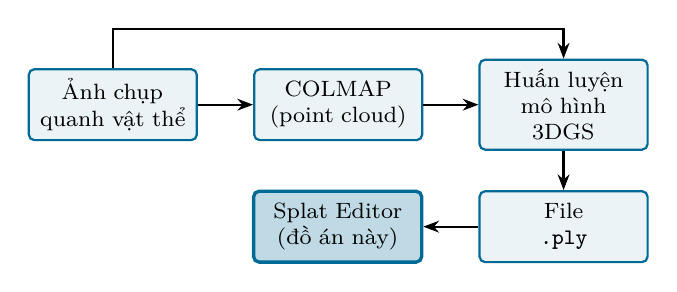
\begin{tikzpicture}[
  node distance=5mm and 7mm,
  box/.style={draw=linkblue,thick,rounded corners=2pt,fill=linkblue!8,align=center,
              minimum height=9mm,text width=19mm,font=\footnotesize},
  mine/.style={box,fill=linkblue!25,very thick},
  arr/.style={-{Stealth[length=2mm]},thick}]
  \node[box] (photos) {Ảnh chụp\\quanh vật thể};
  \node[box,right=of photos] (colmap) {COLMAP\\(point cloud)};
  \node[box,right=of colmap] (train) {Huấn luyện\\mô hình 3DGS};
  \node[box,below=of train] (ply) {File\\\code{.ply}};
  \node[mine,left=of ply] (editor) {Splat Editor\\(đồ án này)};
  \draw[arr] (photos) -- (colmap);
  \draw[arr] (colmap) -- (train);
  \draw[arr] (photos.north) -- ++(0,5mm) -| (train.north);
  \draw[arr] (train) -- (ply);
  \draw[arr] (ply) -- (editor);
\end{tikzpicture}
\caption{Quy trình từ ảnh chụp đến Splat Editor. COLMAP \cite{schonberger2016colmap} tìm vị trí các camera.}
\label{fig:pipeline}
\end{figure}

Đồ án có hai phần. Phần một là pipeline hiển thị 3DGS, từ file đến shader. Phần hai là sáu nhóm kỹ thuật của môn học (Bảng~\ref{tab:map}).

\begin{table}[H]
\centering
\caption{Các nhóm kỹ thuật và các mục.}
\label{tab:map}
\footnotesize
\begin{tabular}{@{}lll@{}}
\toprule
Nhóm & Nội dung chính & Mục \\
\midrule
T1 & layer, ma trận $\mathbf{M}$ & \ref{chap:t1} \\
T2 & ma trận nhìn/chiếu, EWA, trộn alpha, camera & \ref{chap:t2} \\
T3 & texture skin của nhân vật & \ref{chap:t3} \\
T4 & màu SH, Phong, shadow map & \ref{chap:t4} \\
T5 & chu kỳ ngày đêm, va chạm, người chơi & \ref{chap:t5} \\
T6 & cọ chọn, xóa/hoàn tác, ImGui, HUD & \ref{chap:t6} \\
\bottomrule
\end{tabular}
\end{table}

\subsection{Cấu trúc chương trình}
Mã nguồn chia theo vai trò. \code{core} chỉ chứa dữ liệu và toán nên không phụ thuộc OpenGL. \code{render} chứa mọi lệnh OpenGL và shader. \code{ui} lo giao diện, còn \code{app.py} nối các phần lại. Hình~\ref{fig:tree} liệt kê các file chính.

\begin{figure}[H]
\centering
\begin{Verbatim}[fontsize=\fontsize{5.6}{6.6}\selectfont,frame=single]
SplatOpenGL/
|-- main.py              # điểm vào: python main.py [scene.ply]
|-- requirements.txt     # numpy, PyOpenGL, glfw, imgui-bundle
`-- splat_editor/
    |-- app.py           # vòng lặp chính, nối các phần lại
    |-- core/            # dữ liệu và toán, không dùng OpenGL
    |   |-- splats.py    # các mảng gaussian
    |   |-- layer.py     # một file PLY + biến đổi + vùng chọn
    |   |-- scene.py     # tập các layer
    |   |-- math3d.py    # ma trận V, P, góc Euler, quaternion
    |   |-- lighting.py  # mặt trời, đèn, ngày đêm
    |   |-- physics.py   # va chạm voxel, nhảy
    |   |-- avatar_pose.py  # góc khớp nhân vật
    |   |-- lod.py       # chọn gaussian theo mức chi tiết
    |   `-- history.py   # hoàn tác (undo)
    |-- io/              # đọc / ghi file
    |   |-- ply.py       # đọc / ghi PLY
    |   `-- codec.py     # cột PLY <-> Splats
    |-- editor/          # chỉnh sửa
    |   |-- editor.py    # mở, lưu, xoá, chọn
    |   `-- brush.py     # cọ chọn gaussian
    |-- render/          # OpenGL
    |   |-- splat_renderer.py  # vẽ gaussian (2 pass)
    |   |-- sorter.py    # sắp xếp độ sâu (luồng nền)
    |   |-- camera.py    # camera quỹ đạo / bay
    |   |-- avatar_renderer.py # vẽ nhân vật
    |   |-- shader.py    # biên dịch GLSL
    |   |-- shaders/     # splat_prep.vert, splat.vert/.frag, ...
    |   `-- textures/    # skinzom.png
    `-- ui/              # giao diện ImGui
        |-- window.py    # cửa sổ GLFW
        |-- input.py     # bàn phím, chuột
        `-- sections.py  # các bảng điều khiển
\end{Verbatim}
\caption{Cây thư mục của chương trình (chỉ các file chính).}
\label{fig:tree}
\end{figure}

\subsection{Dữ liệu đầu vào}
\label{sec:input}
Đầu vào là một file \code{.ply} do quá trình huấn luyện 3DGS tạo ra. Huấn luyện bắt đầu từ point cloud của COLMAP và đặt một gaussian tại mỗi điểm. Sau đó nó lặp lại ba bước: vẽ các gaussian, so ảnh vẽ ra với ảnh chụp thật, rồi cập nhật tham số của từng gaussian. Trong lúc đó nó cũng xóa các gaussian vô ích và tách các gaussian quá lớn.

File gồm header dạng văn bản và phần thân nhị phân. Header liệt kê các thuộc tính, còn phần thân có một bản ghi cho mỗi gaussian. Mỗi giá trị là một số thực 32 bit (Bảng~\ref{tab:ply}). Với SH bậc 3, một bản ghi có 62 giá trị, tức 248 byte. Hình~\ref{fig:csv} là các dòng đầu của một file, xuất ra CSV.

\begin{table}[H]
\centering
\caption{Các thuộc tính của một gaussian trong file PLY.}
\label{tab:ply}
\footnotesize
\begin{tabular}{@{}p{2.3cm}p{0.9cm}p{4.4cm}@{}}
\toprule
Thuộc tính & Số & Ý nghĩa \\
\midrule
\code{x, y, z} & 3 & tâm $\symbf{\mu}$ \\
\code{nx, ny, nz} & 3 & pháp tuyến, luôn bằng 0, không dùng \\
\code{f\_dc\_0..2} & 3 & màu cơ bản (SH bậc 0) \\
\code{f\_rest\_*} & 45 & hệ số SH bậc 1 đến 3 \\
\code{opacity} & 1 & độ đục thô \\
\code{scale\_0..2} & 3 & logarit của kích thước \\
\code{rot\_0..3} & 4 & quaternion quay \\
\bottomrule
\end{tabular}
\end{table}

\begin{figure}[H]
\centering
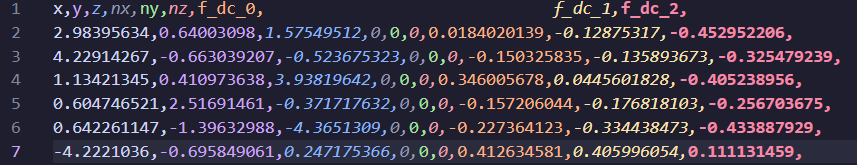
\includegraphics[width=\columnwidth]{figures/csv_head.png}\\[2pt]
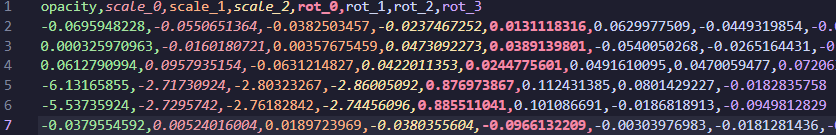
\includegraphics[width=\columnwidth]{figures/csv_tail.png}
\caption{Sáu gaussian đầu tiên của một file PLY, hiển thị dạng CSV. Trên: vị trí, pháp tuyến và màu cơ bản. Dưới: độ đục, kích thước và phép quay. Các cột \code{f\_rest} ở giữa được ẩn đi.}
\label{fig:csv}
\end{figure}

Chương trình ánh xạ file nhị phân thẳng vào bộ nhớ, nên file có hàng triệu gaussian vẫn mở gần như tức thì. Hình~\ref{fig:viewer} là một bản chụp nhỏ của một người. Các đốm mờ quanh người là gaussian lơ lửng mà trình chỉnh sửa phải xóa. Cảnh thử nghiệm chính là một con phố có khoảng 5 triệu gaussian (Hình~\ref{fig:scene}).

\begin{figure}[H]
\centering
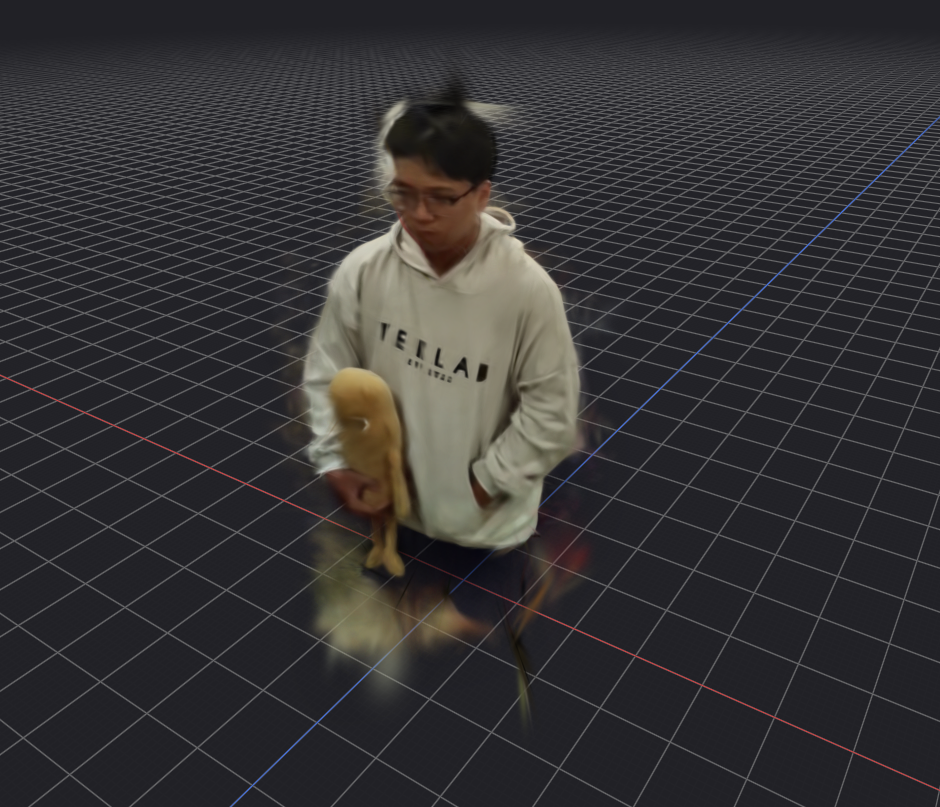
\includegraphics[width=0.6\columnwidth]{figures/viewer.png}
\caption{File PLY của một người được chụp lại. Các gaussian lơ lửng hiện rõ quanh người và gần mặt đất.}
\label{fig:viewer}
\end{figure}

\begin{figure}[H]
\centering
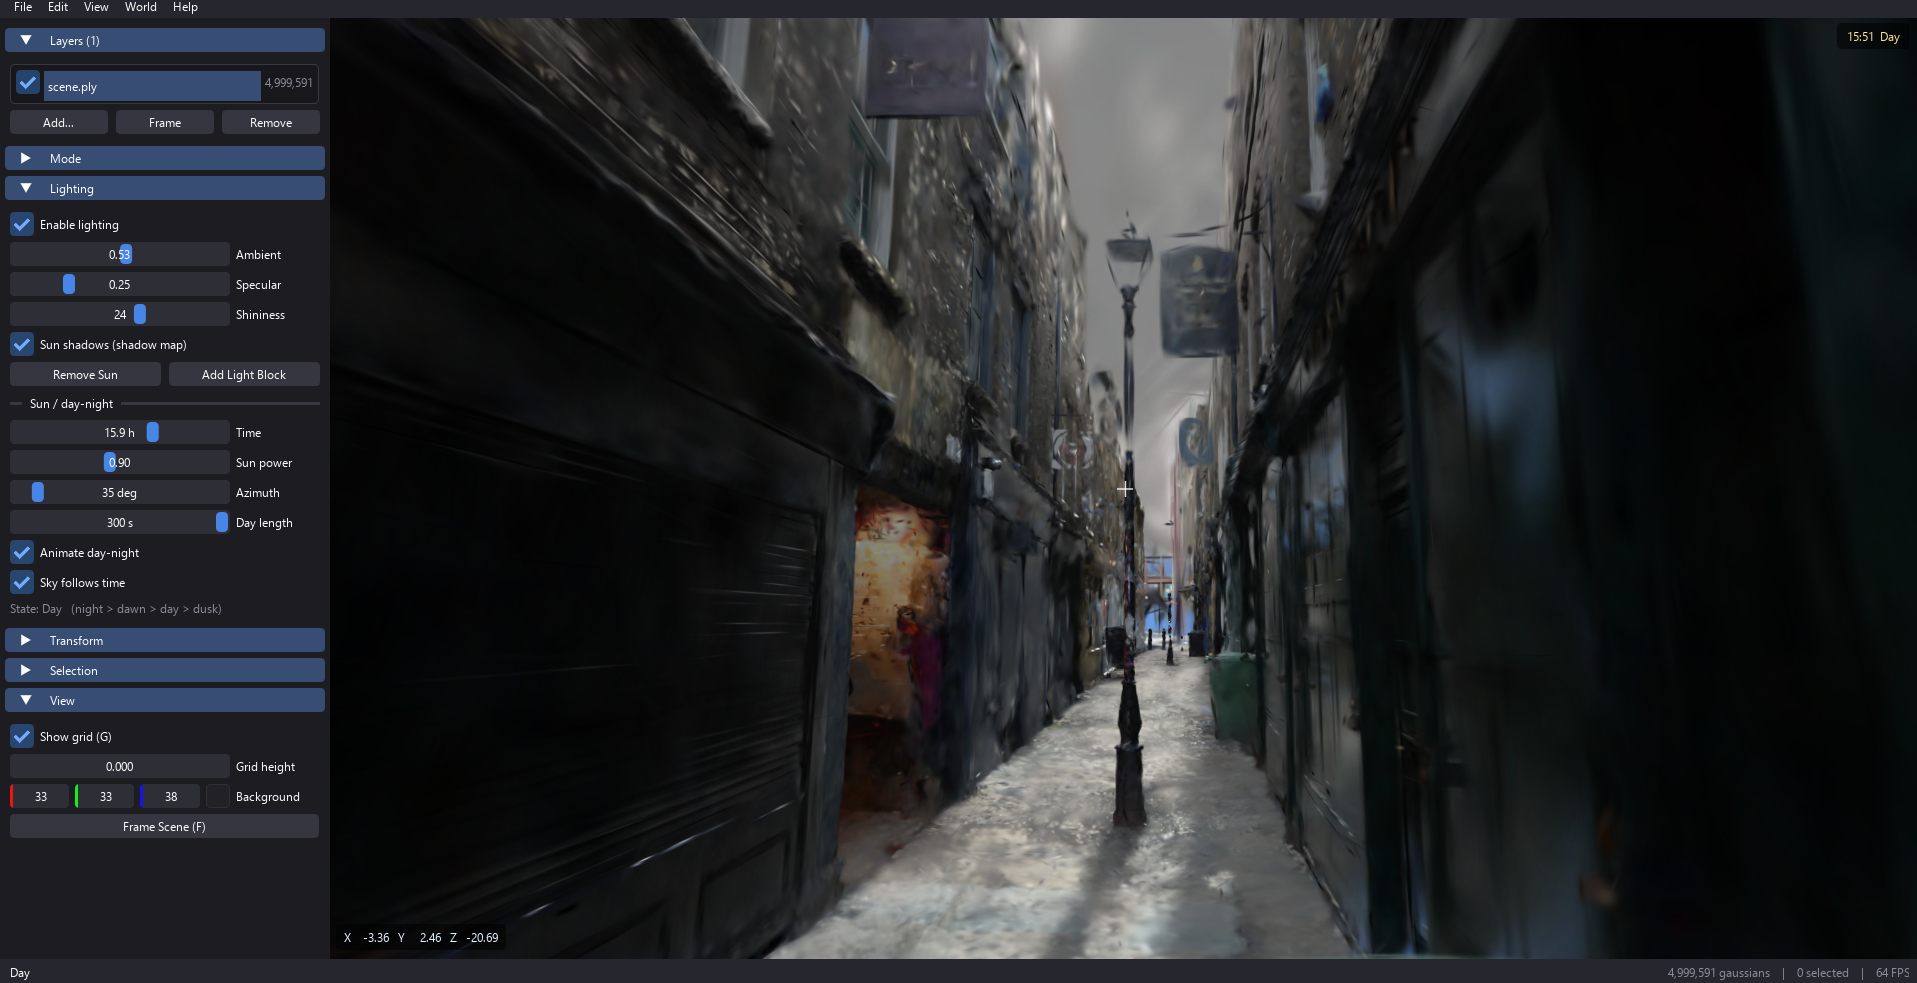
\includegraphics[width=\columnwidth]{figures/t4-day.png}\\[3pt]
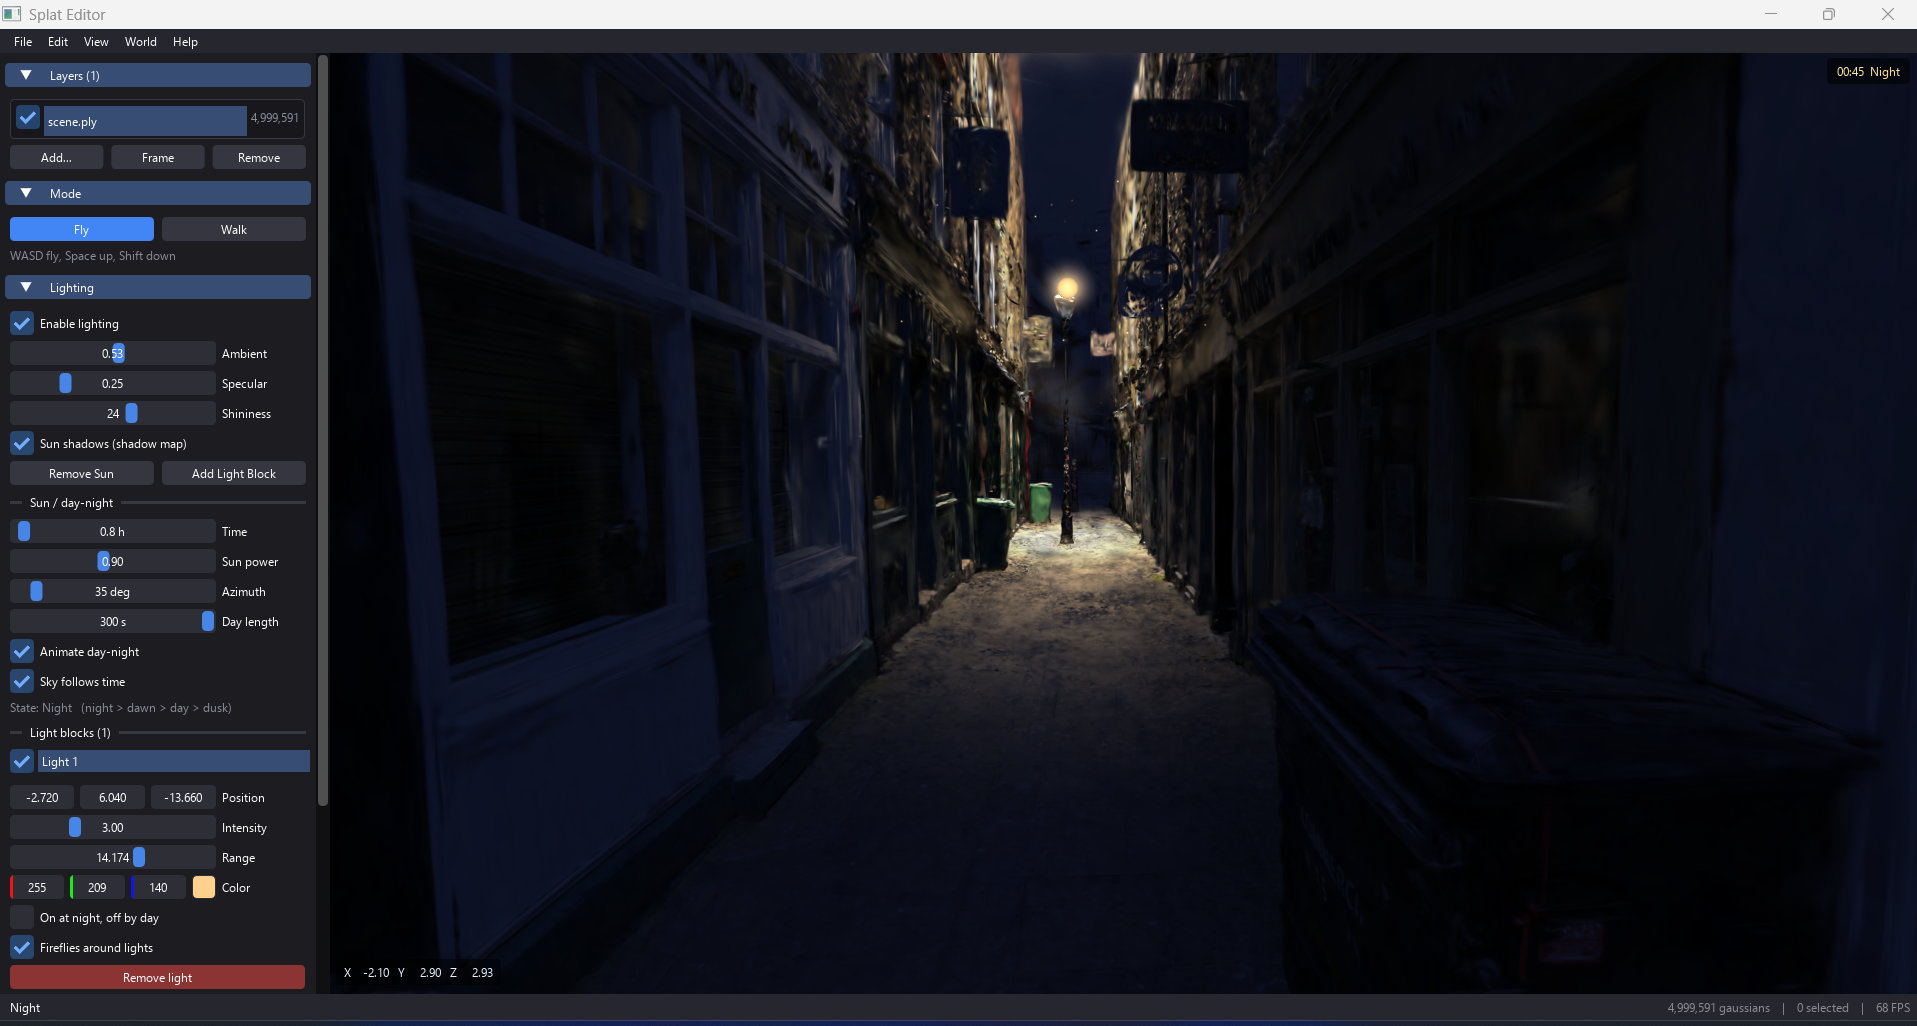
\includegraphics[width=\columnwidth]{figures/t4-night.png}
\caption{Một cảnh khoảng 5 triệu gaussian trong Splat Editor, ban ngày (trên) và ban đêm (dưới).}
\label{fig:scene}
\end{figure}

\subsection{Gaussian và file PLY}
\label{sec:decode}
Mỗi gaussian có vị trí $\symbf{\mu}$, màu $\mathbf{c}$, độ đục $\alpha$, kích thước $\mathbf{s}$ và phép quay $\symbf{q}$ (một quaternion). Mật độ của nó giảm dần từ tâm ra ngoài, nên có thể hình dung nó là một ellipsoid (Hình~\ref{fig:g2e}). File PLY lưu giá trị thô, chương trình giải mã khi đọc:
\begin{itemize}\itemsep0pt
  \item Kích thước: $s_i=\exp(\code{scale\_i})$.
  \item Độ đục: $\alpha=1/(1+e^{-\code{opacity}})$.
  \item Màu: $\mathrm{RGB}=0{,}5+C_0\,\code{f\_dc}$, với $C_0\approx0{,}2821$.
  \item Phép quay: chuẩn hóa quaternion \code{rot\_0..3} về độ dài 1.
\end{itemize}
Khi lưu file, chương trình áp dụng công thức ngược lại.

\par\noindent\fcolorbox{red}{white}{\footnotesize\textbf{Mã nguồn: Listing~\ref{lst:decode} (Phụ lục~\ref{app:code}).}}\par\vspace{3pt}

\begin{figure}[H]
\centering
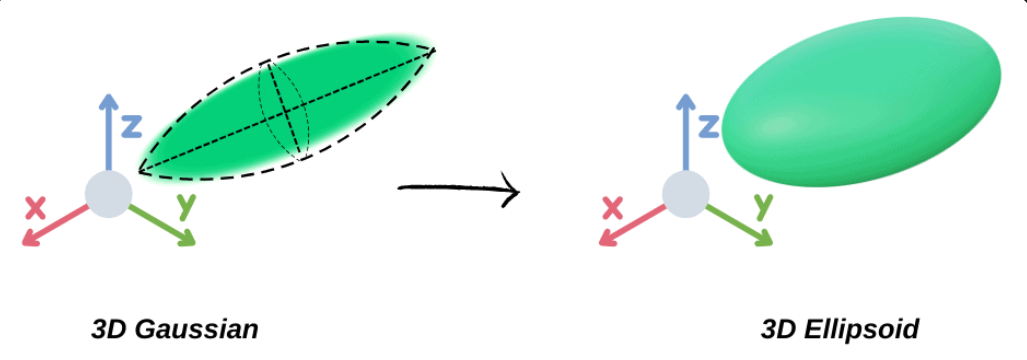
\includegraphics[width=\columnwidth]{figures/1 (4).png}
\caption{Gaussian 3D là một đốm mềm. Mặt của nó tại một độ lệch chuẩn là một ellipsoid.}
\label{fig:g2e}
\end{figure}

Ma trận hiệp phương sai $\Sig$ chứa hình dạng của gaussian. Nó được tạo từ ma trận co giãn $\mathbf{S}=\mathrm{diag}(\mathbf{s})$ và ma trận quay $\mathbf{R}(\symbf{q})$:
\begin{equation}
\Sig=\mathbf{R}\,\mathbf{S}\mathbf{S}^{\top}\mathbf{R}^{\top}.
\label{eq:cov3d}
\end{equation}
Hình~\ref{fig:rs} cho hai ma trận này, còn Hình~\ref{fig:ellipsoid} vẽ kết quả cho gaussian đầu tiên của Hình~\ref{fig:csv}. Ba kích thước $s_0,s_1,s_2$ là các bán trục của ellipsoid, và quaternion xoay các trục này trong không gian. Mục~\ref{sec:ewa} chiếu ellipsoid này lên màn hình.

\par\noindent\fcolorbox{red}{white}{\footnotesize\textbf{Mã nguồn: Listing~\ref{lst:cov3d} (Phụ lục~\ref{app:code}).}}\par\vspace{3pt}

\begin{figure}[H]
\centering
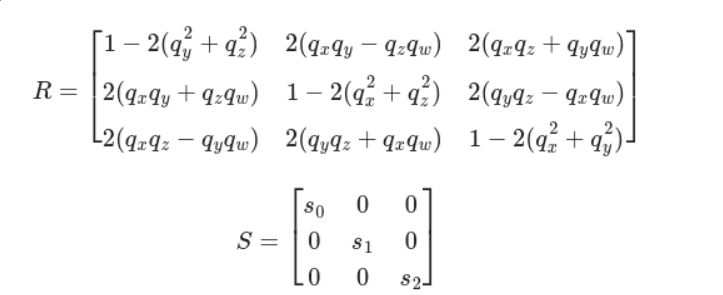
\includegraphics[width=0.75\columnwidth]{figures/1 (5).png}
\caption{Ma trận quay $\mathbf{R}$ từ quaternion $(q_w,q_x,q_y,q_z)$ và ma trận co giãn $\mathbf{S}$.}
\label{fig:rs}
\end{figure}

\begin{figure}[H]
\centering
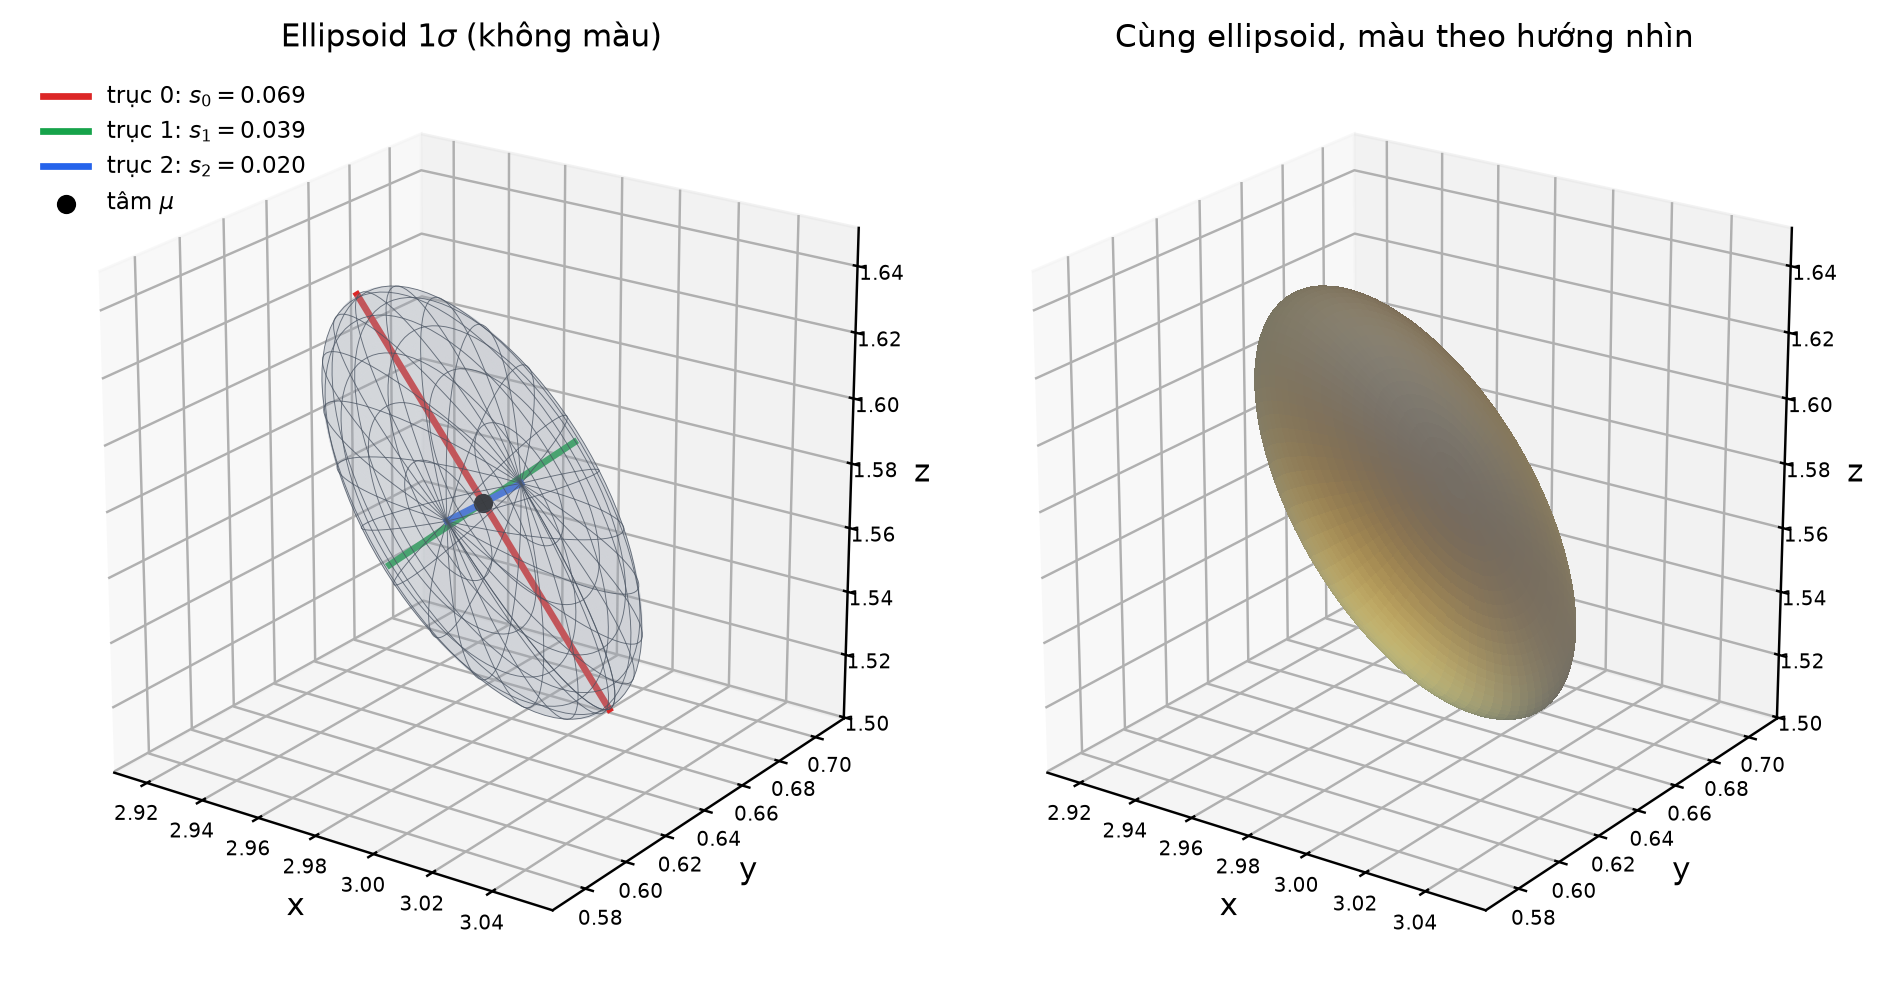
\includegraphics[width=\columnwidth]{figures/example_ellipsoid.png}
\caption{Một gaussian trong file. Trái: ellipsoid $1\sigma$ với ba trục và tâm $\symbf{\mu}$. Phải: cùng ellipsoid đó với màu phụ thuộc hướng nhìn.}
\label{fig:ellipsoid}
\end{figure}


\begin{figure*}[t]
\centering
\begin{minipage}{0.495\textwidth}\centering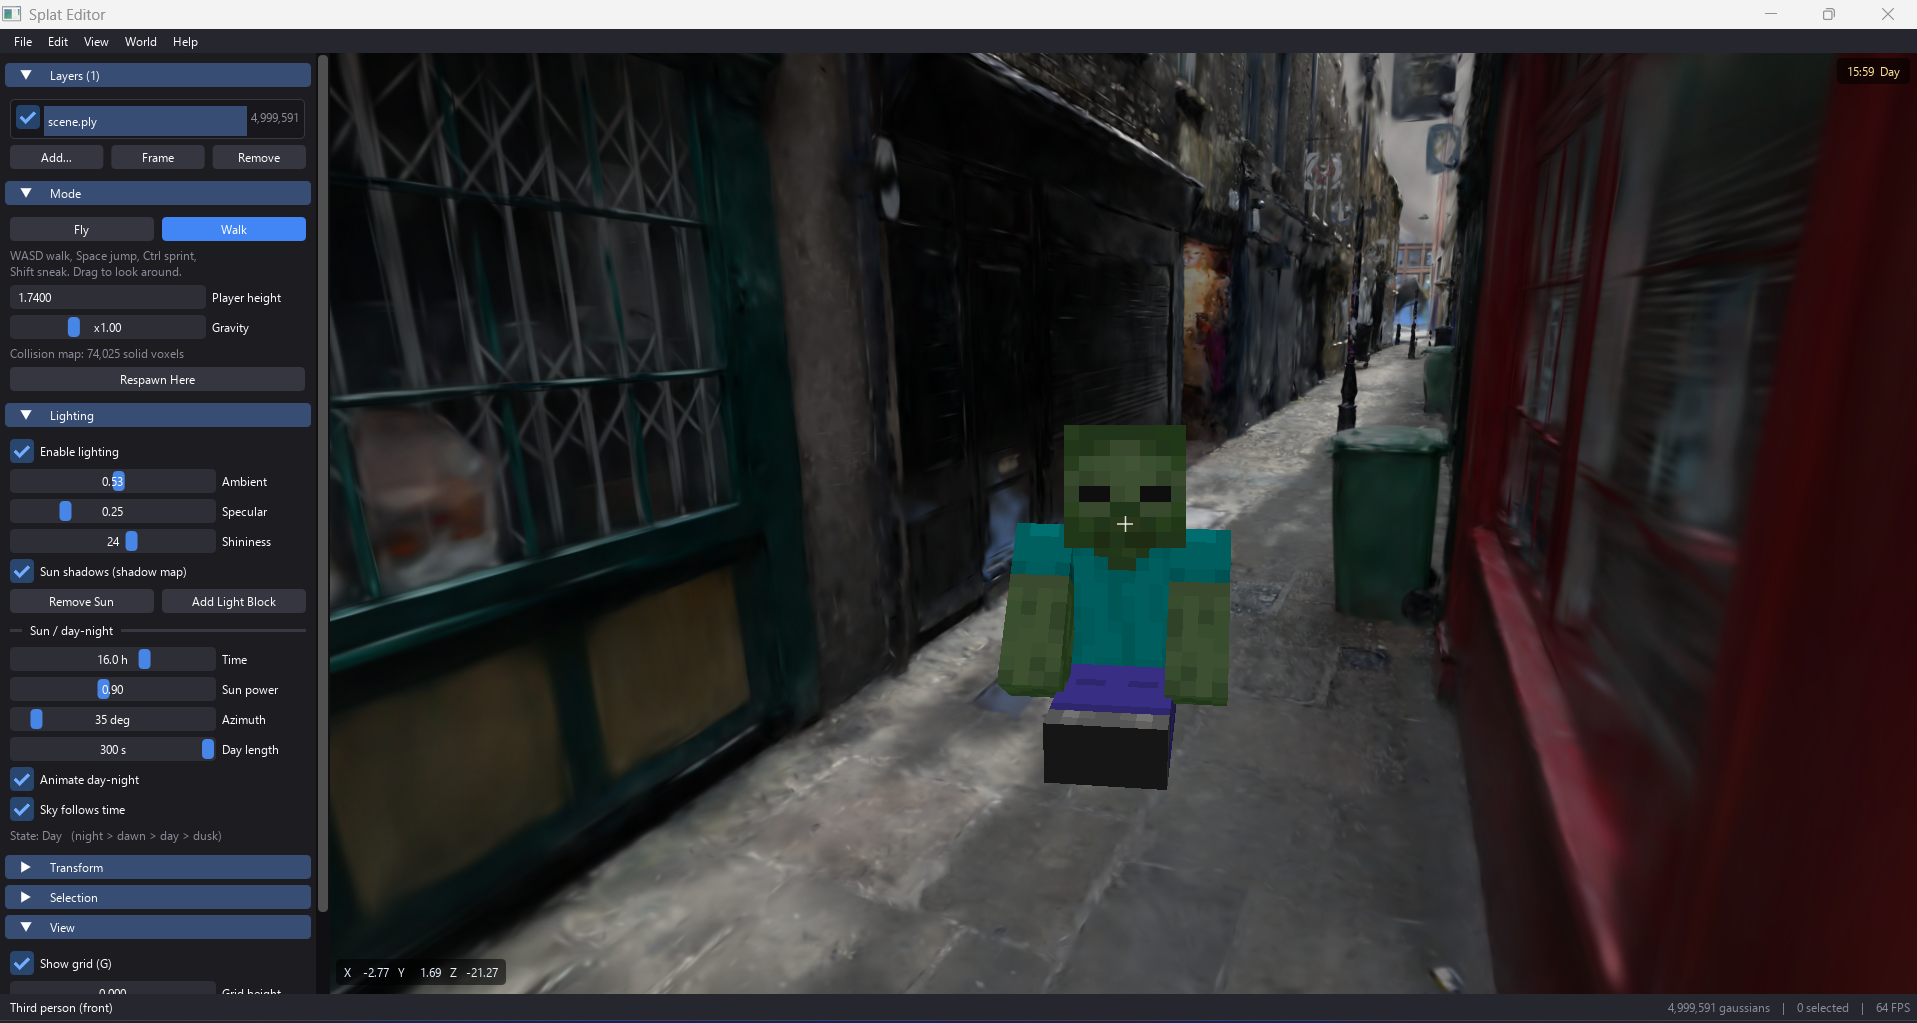
\includegraphics[width=\linewidth]{figures/t4-zombie-day.png}\\{\footnotesize (a) Ban ngày, 15:59.}\end{minipage}\hfill
\begin{minipage}{0.495\textwidth}\centering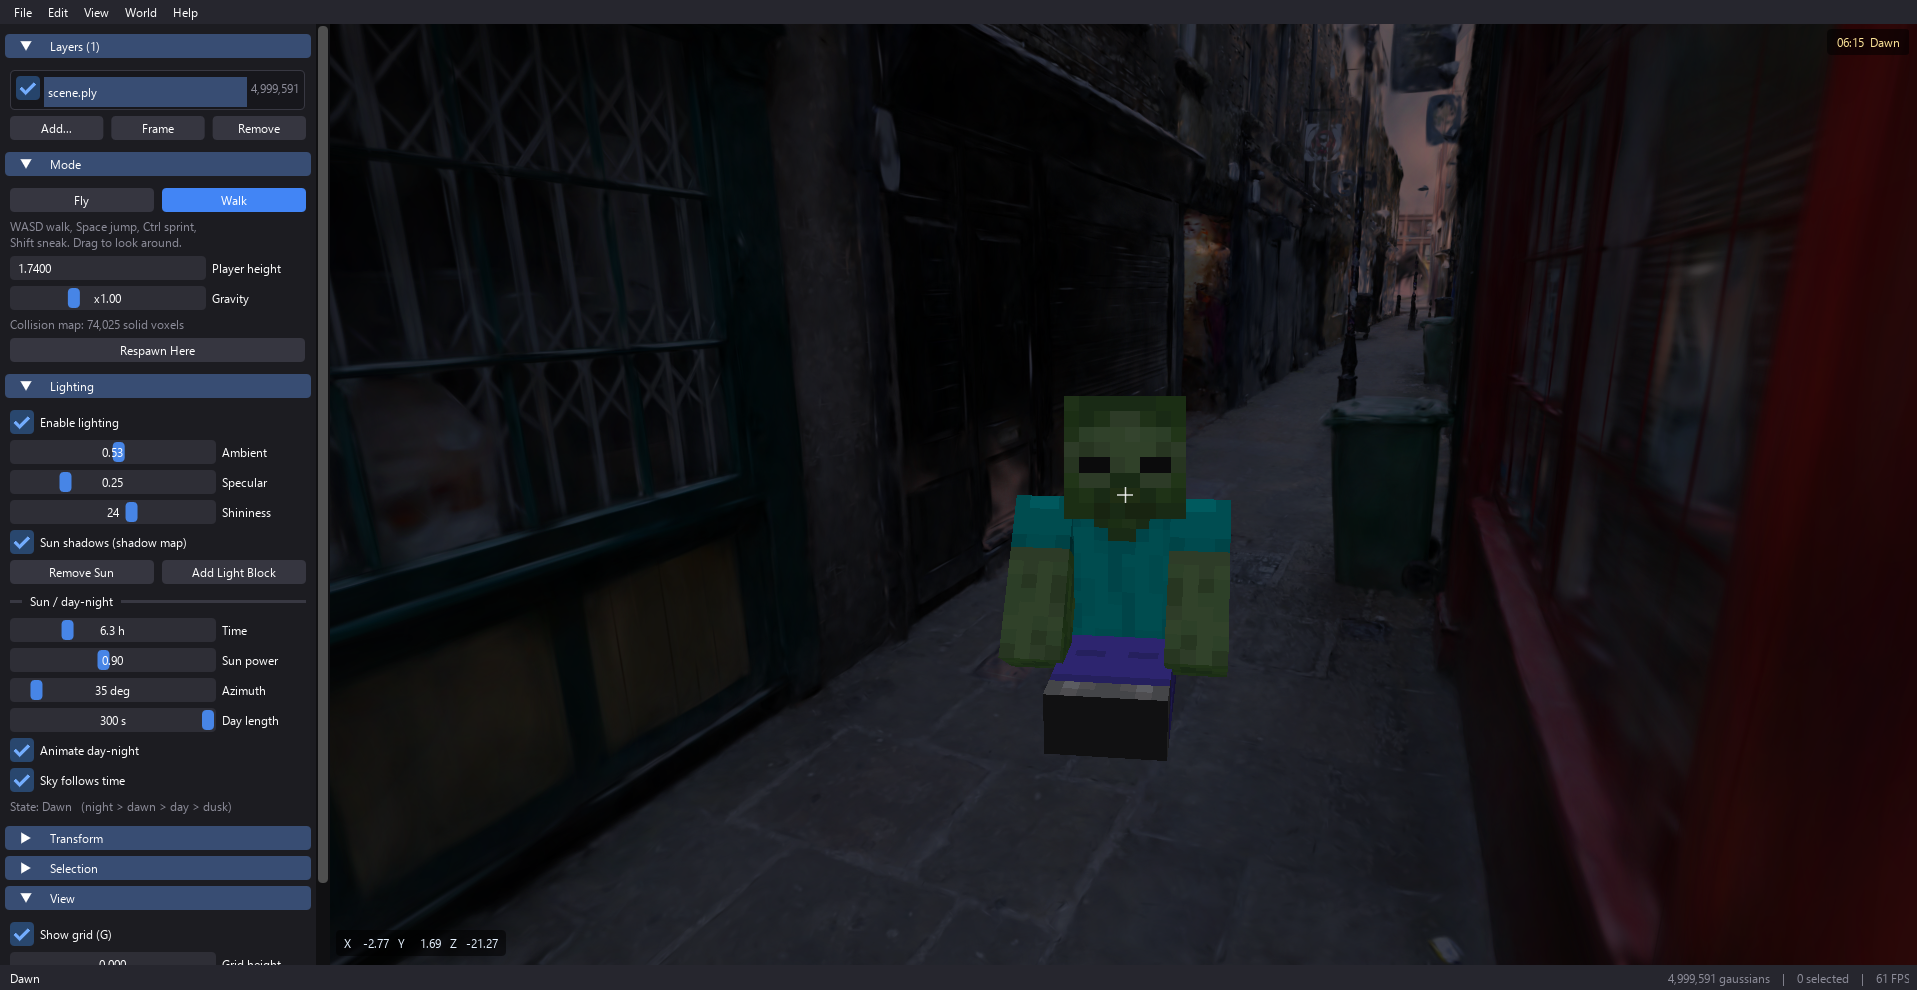
\includegraphics[width=\linewidth]{figures/t4-dawn.png}\\{\footnotesize (b) Bình minh, 06:15.}\end{minipage}\\[5pt]
\begin{minipage}{0.495\textwidth}\centering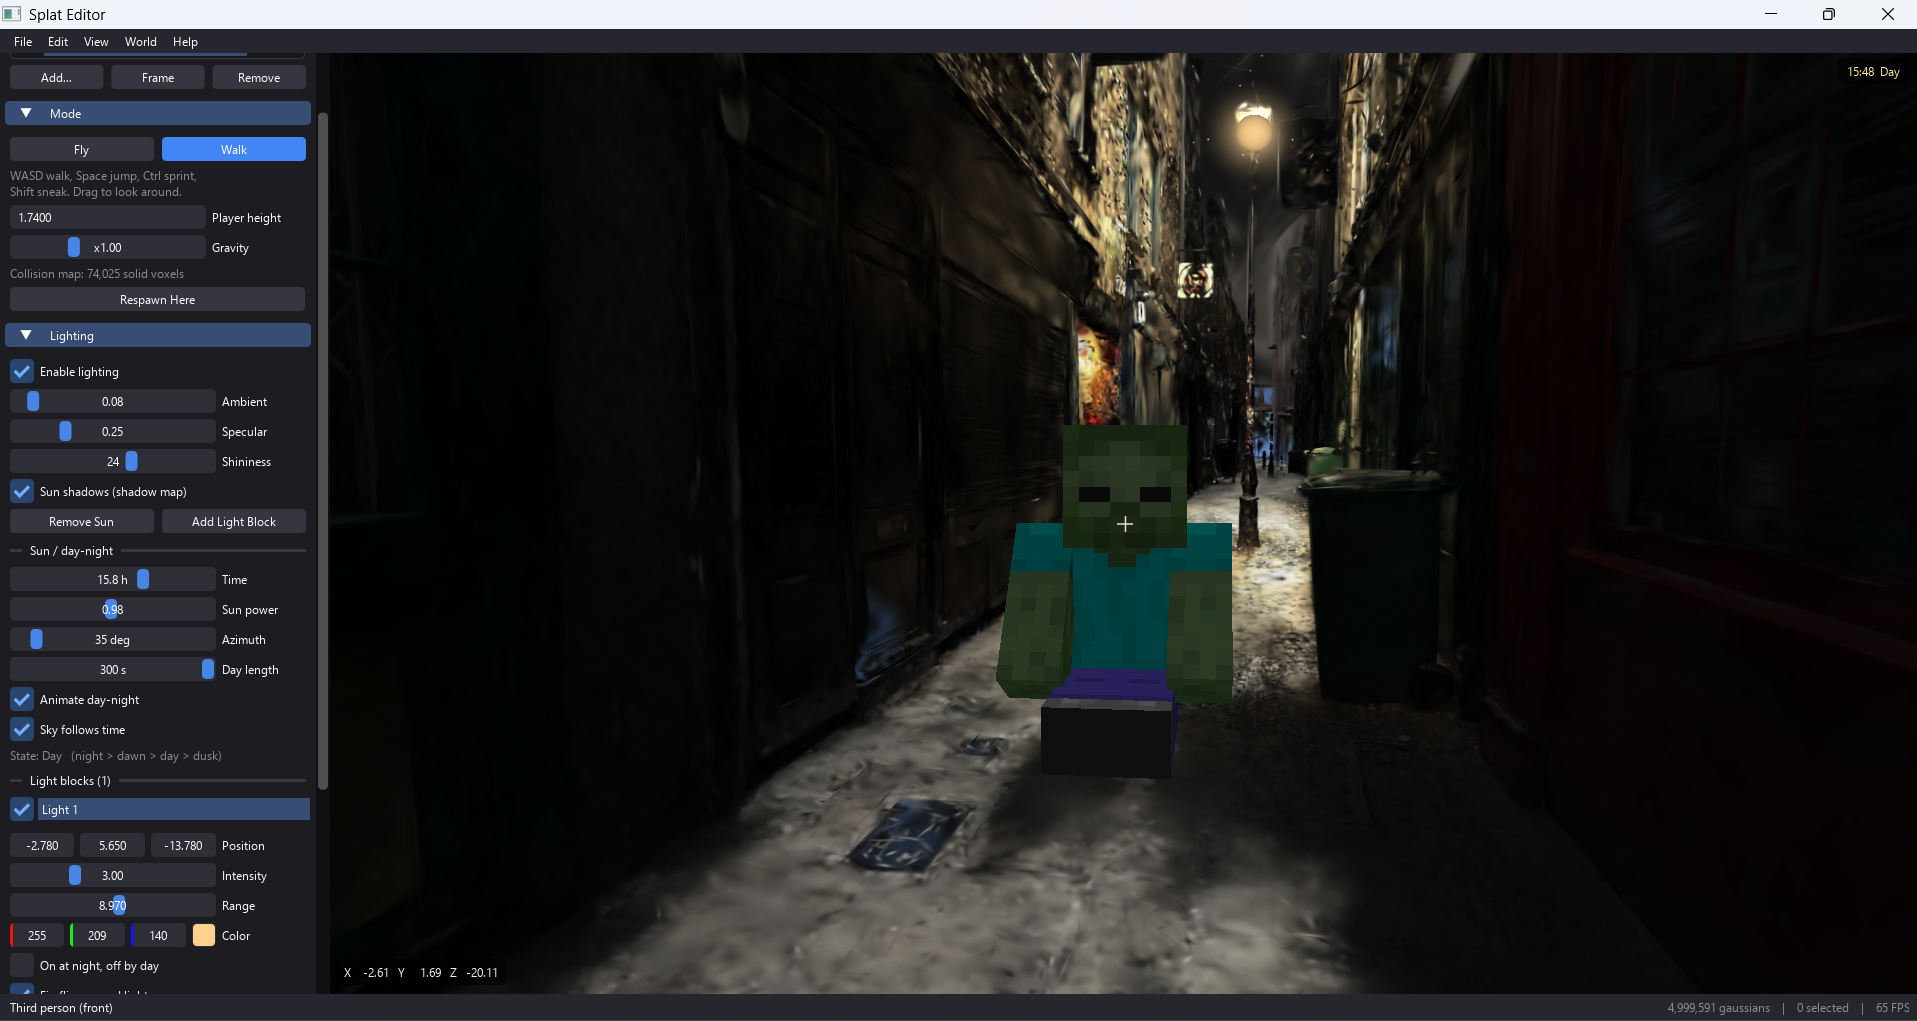
\includegraphics[width=\linewidth]{figures/t4-lamp-zombie.png}\\{\footnotesize (c) Môi trường $0{,}08$ và một đèn.}\end{minipage}\hfill
\begin{minipage}{0.495\textwidth}\centering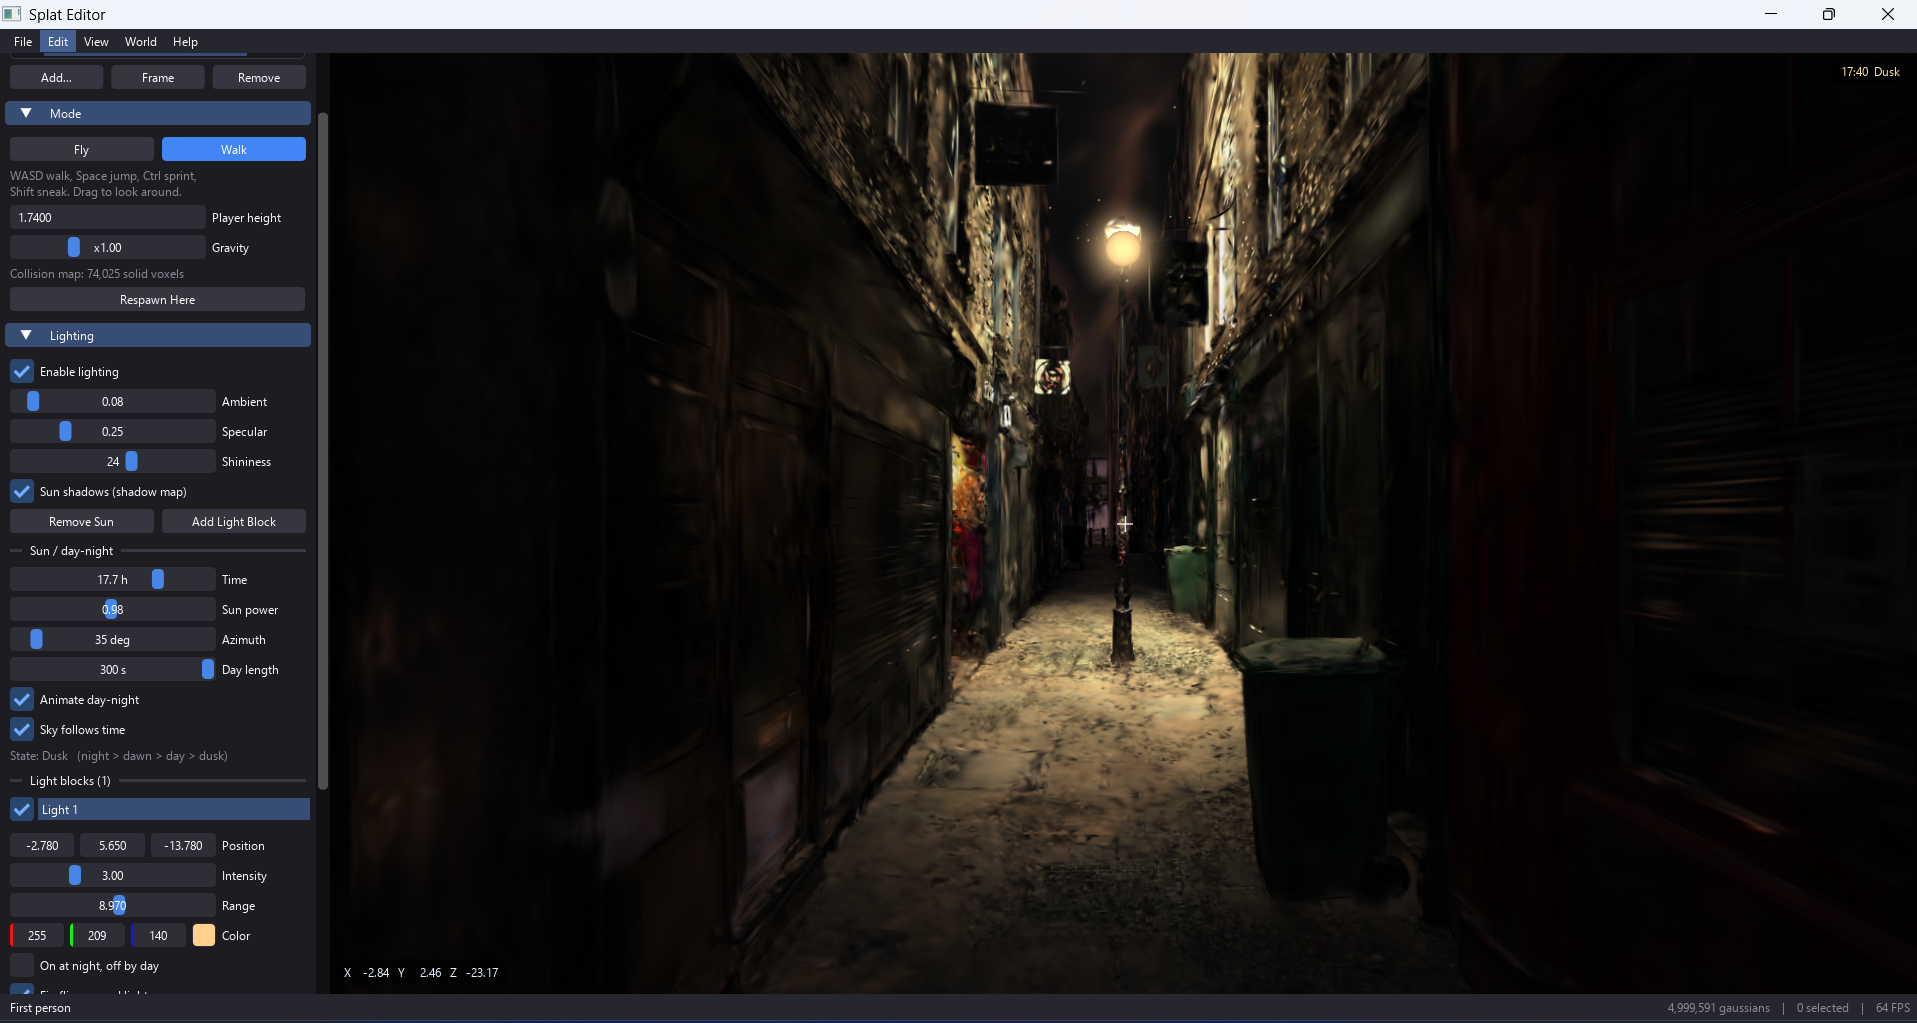
\includegraphics[width=\linewidth]{figures/t4-dusk.png}\\{\footnotesize (d) Hoàng hôn, 17:40.}\end{minipage}
\caption{Cảnh có mặt trời, một đèn điểm và nhân vật vào các giờ khác nhau trong ngày.}
\label{fig:t4}
\end{figure*}


%====================================================================
\section{T1: Phép biến đổi và mô hình phân cấp}
\label{chap:t1}
%====================================================================
Mục này có hai phần, cả hai đều di chuyển cả một layer.
\begin{itemize}\itemsep0pt
\item Phần 1, biến đổi layer: đặt các gaussian của một file \code{.ply} vào thế giới.
\item Phần 2, quay quanh một điểm: quay layer quanh một tâm tùy chọn.
\end{itemize}

\subsection{Phần 1: Biến đổi layer}
\label{sec:layers}
Mỗi file \code{.ply} là một layer. Layer có vector tịnh tiến $\mathbf{t}$, ba góc Euler và hệ số co giãn $s$. Chúng tạo thành ma trận $\mathbf{M}$, đưa gaussian từ không gian file sang không gian thế giới:
\begin{equation}
\mathbf{p}_w=s\mathbf{A}\mathbf{p}_f+\mathbf{t},\qquad
\Sig_w=s^{2}\mathbf{A}\,\Sig_f\,\mathbf{A}^{\top}.
\label{eq:world}
\end{equation}
Ở đây $\mathbf{A}=\mathbf{R}_z\mathbf{R}_y\mathbf{R}_x\mathbf{F}$, với $\mathbf{F}=\mathrm{diag}(-1,-1,1)$ là phép lật tùy chọn cho file COLMAP có trục $Y$ hướng xuống. Di chuyển, xoay hay co giãn một layer chỉ đổi $\mathbf{M}$ và giữ nguyên dữ liệu gaussian, nên diễn ra tức thì. Khi lưu, chương trình ghi phép biến đổi vào từng gaussian. Nó cũng xoay các hệ số SH để màu theo hướng nhìn vẫn đúng.

\par\noindent\fcolorbox{red}{white}{\footnotesize\textbf{Mã nguồn: Listing~\ref{lst:world} (Phụ lục~\ref{app:code}).}}\par\vspace{3pt}

\subsection{Phần 2: Quay quanh một điểm}
Layer cũng có thể quay quanh một điểm $\mathbf{c}$. Với $\symbf{\Delta}$ là ma trận quay:
\begin{equation}
\mathbf{R}'=\symbf{\Delta}\mathbf{R},\qquad \mathbf{t}'=\symbf{\Delta}(\mathbf{t}-\mathbf{c})+\mathbf{c}.
\end{equation}

\par\noindent\fcolorbox{red}{white}{\footnotesize\textbf{Mã nguồn: Listing~\ref{lst:pivot} (Phụ lục~\ref{app:code}).}}\par\vspace{3pt}

%====================================================================
\section{T2: Camera và phép chiếu}
\label{chap:t2}
%====================================================================
Một gaussian đi qua bốn bước để thành pixel trên màn hình \cite{zwicker2002ewa}. Mỗi bước là một ô trong Hình~\ref{fig:ewa}, đọc từ trái sang phải. Phần 5 nói về camera.
\begin{itemize}\itemsep0pt
\item Phần 1, phép biến đổi nhìn (\emph{viewing transformation}): đưa gaussian từ không gian vật thể về không gian camera.
\item Phần 2, phép chiếu (\emph{projective mapping}): biến ellipsoid 3D thành ellipse 2D.
\item Phần 3, tô màu và trộn (\emph{shading and integration}): tính độ đục tại từng pixel và trộn các gaussian với nhau.
\item Phần 4, phép biến đổi vùng nhìn (\emph{viewport transformation}): đặt kết quả vào vùng nhìn của cửa sổ.
\item Phần 5, hai loại camera: camera cho vị trí mắt và điểm nhìn mà Phần 1 cần.
\end{itemize}
\begin{figure}[H]
\centering
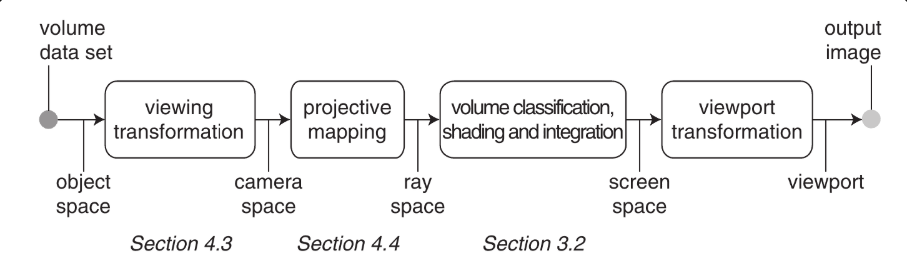
\includegraphics[width=\columnwidth]{figures/1 (3).png}
\caption{Pipeline splatting của EWA \cite{zwicker2002ewa}. Phép biến đổi nhìn là $\mathbf{W}$ và phép chiếu được xấp xỉ bằng $\mathbf{J}$.}
\label{fig:ewa}
\end{figure}

\subsection{Phần 1: Phép biến đổi nhìn}
\label{sec:cam}
Bước này đổi hệ tọa độ sao cho camera nằm ở gốc và nhìn dọc theo trục $-z$. Hàm \code{look\_at} tạo ba trục camera từ vị trí mắt $\mathbf{e}$ và điểm nhìn: phải $\mathbf{r}$, lên $\mathbf{u}$ và trước $\mathbf{f}$. Ma trận nhìn là
\begin{equation}
\mathbf{V}=\begin{pmatrix}
\setlength{\fboxsep}{2pt}\fcolorbox{red}{white}{$\begin{matrix}
r_x&r_y&r_z\\u_x&u_y&u_z\\-f_x&-f_y&-f_z\end{matrix}$}
&\begin{matrix}-\mathbf{r}\!\cdot\!\mathbf{e}\\-\mathbf{u}\!\cdot\!\mathbf{e}\\ \mathbf{f}\!\cdot\!\mathbf{e}\end{matrix}\\[3mm]
\begin{matrix}0&0&0\end{matrix}&1\end{pmatrix}.
\label{eq:view}
\end{equation}
Nhân tâm gaussian với $\mathbf{V}$ cho tâm trong không gian camera, $(v_x,v_y,v_z)$. Hình dạng của gaussian thì chỉ bị quay, bằng ma trận $\mathbf{W}$. $\mathbf{W}$ là phần quay của $\mathbf{V}$: khối $3\times3$ trên trái, nằm trong khung đỏ ở \eqref{eq:view}. Các hàng của nó là ba trục camera:
\begin{equation}
\mathbf{W}=\begin{pmatrix}
r_x&r_y&r_z\\u_x&u_y&u_z\\-f_x&-f_y&-f_z\end{pmatrix}.
\label{eq:W}
\end{equation}
Trong không gian camera, ellipsoid \eqref{eq:cov3d} trở thành $\mathbf{W}\,\Sig\,\mathbf{W}^{\top}$.

\par\noindent\fcolorbox{red}{white}{\footnotesize\textbf{Mã nguồn: Listing~\ref{lst:lookat} (Phụ lục~\ref{app:code}).}}\par\vspace{3pt}

\subsection{Phần 2: Phép chiếu}
\label{sec:ewa}
Bước này đưa gaussian từ không gian camera lên mặt phẳng ảnh.

\textbf{Chiếu một điểm.} Ma trận chiếu phối cảnh dùng góc nhìn dọc $\varphi$ ($k=1/\tan(\varphi/2)$), tỉ lệ khung hình $a$, mặt phẳng gần $n$ và xa $f$:
\begin{equation}
\mathbf{P}=\begin{pmatrix}
\frac{k}{a}&0&0&0\\0&k&0&0\\
0&0&\frac{f+n}{n-f}&\frac{2fn}{n-f}\\0&0&-1&0\end{pmatrix}.
\label{eq:proj}
\end{equation}
Điểm được nhân với $\mathbf{P}$ rồi chia cho $c_w$. Kết quả là tọa độ chuẩn hóa $(n_x,n_y)$ trong khoảng $[-1,1]$. Chính phép chia cho $c_w$ làm vật ở xa trông nhỏ hơn. Tâm gaussian được chiếu theo cách này.

\par\noindent\fcolorbox{red}{white}{\footnotesize\textbf{Mã nguồn: Listing~\ref{lst:persp} (Phụ lục~\ref{app:code}).}}\par\vspace{3pt}

\textbf{Chiếu một gaussian.} Ellipsoid của gaussian phải thành một ellipse trên màn hình. Phép chia cho $c_w$ không tuyến tính, nên không thể nhân thẳng $\mathbf{P}$ với ellipsoid. EWA thay phép chiếu bằng đạo hàm của nó, tức Jacobian, tại tâm gaussian:
\begin{equation}
\mathbf{J}=\begin{pmatrix}
\frac{f_{px}}{-v_z}&0&\frac{f_{px}\,v_x}{v_z^{2}}\\[1mm]
0&\frac{f_{px}}{-v_z}&\frac{f_{px}\,v_y}{v_z^{2}}\\[1mm]
0&0&0
\end{pmatrix}.
\label{eq:jac}
\end{equation}
Ở đây $f_{px}=kH/2$ là tiêu cự tính bằng pixel, với $k$ lấy từ \eqref{eq:proj} và $H$ là chiều cao vùng nhìn. Ghép bước 1 và bước 2 cho hiệp phương sai 2D:
\begin{equation}
\Sig'=\mathbf{J}\,\mathbf{W}\,\Sig\,\mathbf{W}^{\top}\mathbf{J}^{\top}.
\label{eq:ewa}
\end{equation}
Trong công thức này, $\Sig$ là hiệp phương sai 3D \eqref{eq:cov3d}, $\mathbf{W}$ là phần quay của ma trận nhìn ở bước 1 và $\mathbf{J}$ là Jacobian \eqref{eq:jac}. Gọi khối $2\times2$ trên trái của $\Sig'$ là $\begin{pmatrix}a&b\\b&c\end{pmatrix}$. Giá trị riêng của nó là
\begin{equation}
\lambda_{1,2}=\frac{a+c}{2}\pm\sqrt{\Big(\frac{a-c}{2}\Big)^{2}+b^{2}}.
\label{eq:eig}
\end{equation}
Hai bán trục của ellipse tỉ lệ với $\sqrt{\lambda_1}$ và $\sqrt{\lambda_2}$. Shader vẽ mỗi gaussian thành một hình vuông phủ tối đa 3 độ lệch chuẩn. Nó bỏ qua các gaussian có tâm ở sau camera hoặc ngoài màn hình quá $1{,}3$ lần.

\par\noindent\fcolorbox{red}{white}{\footnotesize\textbf{Mã nguồn: Listing~\ref{lst:ewa} (Phụ lục~\ref{app:code}).}}\par\vspace{3pt}

\par\noindent\fcolorbox{red}{white}{\footnotesize\textbf{Mã nguồn: Listing~\ref{lst:eig} (Phụ lục~\ref{app:code}).}}\par\vspace{3pt}

\subsection{Phần 3: Tô màu và trộn alpha}
\label{sec:blend}
Bước này cho mỗi pixel một màu. Với từng pixel $\mathbf{x}$ của hình vuông, fragment shader tính hàm Gaussian 2D. Tâm $\symbf{\mu}'$ là tâm gaussian đã chiếu, còn hiệp phương sai $\Sig'$ lấy từ \eqref{eq:ewa}:
\begin{equation}
G(\mathbf{x})=\exp\!\Big(-\tfrac12(\mathbf{x}-\symbf{\mu}')^{\top}\,\Sig'^{-1}\,(\mathbf{x}-\symbf{\mu}')\Big).
\label{eq:gauss}
\end{equation}
Số mũ bằng $-r^2/2$, với $r$ là khoảng cách đến tâm ellipse đo bằng độ lệch chuẩn. Độ đục của gaussian thứ $i$ tại pixel là $a_i=\alpha_i\,G_i(\mathbf{x})$.

\par\noindent\fcolorbox{red}{white}{\footnotesize\textbf{Mã nguồn: Listing~\ref{lst:frag} (Phụ lục~\ref{app:code}).}}\par\vspace{3pt}

Sau đó các gaussian được trộn theo thứ tự độ sâu. Đánh số các gaussian từ gần đến xa, màu pixel là
\begin{equation}
\mathbf{C}=\sum_{i}\mathbf{c}_i\,a_i\,T_i,\qquad
T_i=\prod_{j<i}(1-a_j),
\label{eq:over}
\end{equation}
trong đó $T_i$ là độ truyền (\emph{transmittance}): phần ánh sáng còn lại sau khi đi qua các gaussian gần hơn $i$.

Chương trình vẽ theo chiều ngược lại, từ xa đến gần. Nó cho cùng kết quả bằng phép trộn $\mathbf{C}\leftarrow\mathbf{c}\,a+(1-a)\,\mathbf{C}$ cho từng splat, với $\mathbf{C}$ là màu đã tích lũy.

Kết quả phụ thuộc thứ tự, nên phải sắp xếp các gaussian theo độ sâu. Chương trình đổi độ sâu thành khóa 16 bit rồi sắp xếp bằng NumPy trong một luồng nền. Khi chưa sắp xếp xong, nó vẽ tạm theo thứ tự của lần trước. Depth test được tắt, vì gaussian trong suốt không được che mất gaussian phía sau.

\par\noindent\fcolorbox{red}{white}{\footnotesize\textbf{Mã nguồn: Listing~\ref{lst:blend} (Phụ lục~\ref{app:code}).}}\par\vspace{3pt}

\par\noindent\fcolorbox{red}{white}{\footnotesize\textbf{Mã nguồn: Listing~\ref{lst:sort} (Phụ lục~\ref{app:code}).}}\par\vspace{3pt}

\subsection{Phần 4: Phép biến đổi vùng nhìn}
\label{sec:viewport}
Bước cuối đổi tọa độ chuẩn hóa $(n_x,n_y)$ của bước 2 sang pixel. Với vùng nhìn kích thước $W\times H$ và góc $(x_0,y_0)$:
\begin{equation}
x_{px}=x_0+\tfrac{n_x+1}{2}W,\qquad y_{px}=y_0+\tfrac{1-n_y}{2}H.
\label{eq:pixel}
\end{equation}
OpenGL tự làm bước này khi vẽ. Chương trình dùng cùng công thức để biết một gaussian rơi vào pixel nào, ví dụ khi chọn bằng cọ (Mục~\ref{chap:t6}).

\par\noindent\fcolorbox{red}{white}{\footnotesize\textbf{Mã nguồn: Listing~\ref{lst:pixel} (Phụ lục~\ref{app:code}).}}\par\vspace{3pt}

\subsection{Phần 5: Hai loại camera}
\textbf{Camera quỹ đạo.} Camera luôn nhìn vào điểm $\mathbf{t}$. Vị trí của nó tính từ góc yaw $\theta$, góc pitch $\phi$ và khoảng cách $d$:
\begin{equation}
\mathbf{e}=\mathbf{t}+d\,(\cos\phi\sin\theta,\ \sin\phi,\ \cos\phi\cos\theta).
\label{eq:eye}
\end{equation}
Pitch bị giới hạn ở khoảng $\pm89^{\circ}$ để camera không lật.

\par\noindent\fcolorbox{red}{white}{\footnotesize\textbf{Mã nguồn: Listing~\ref{lst:eye} (Phụ lục~\ref{app:code}).}}\par\vspace{3pt}

\textbf{Camera bay.} Vận tốc tiến dần đến vận tốc mong muốn $\mathbf{v}^{*}$, nhờ đó camera có quán tính:
\begin{equation}
\mathbf{v}\leftarrow\mathbf{v}+(\mathbf{v}^{*}-\mathbf{v})\min(10\Delta t,1),\qquad
\mathbf{e}\leftarrow\mathbf{e}+\mathbf{v}\,\Delta t.
\label{eq:fly}
\end{equation}

\par\noindent\fcolorbox{red}{white}{\footnotesize\textbf{Mã nguồn: Listing~\ref{lst:fly} (Phụ lục~\ref{app:code}).}}\par\vspace{3pt}


%====================================================================
\section{T3: Ánh xạ texture}
\label{chap:t3}
%====================================================================
Texture phủ ảnh skin lên mô hình hộp của nhân vật. Nhân vật gồm 6 hộp: đầu, thân, hai tay và hai chân. Skin là một ảnh $64\times64$ (Hình~\ref{fig:skin}) chứa hình trải phẳng của cả 6 hộp theo kiểu chữ thập Minecraft. Mỗi mặt hộp chỉ cần lấy đúng ô của nó trên ảnh. Việc vẽ gồm ba bước (Hình~\ref{fig:skinflow}).

\begin{figure}[H]
\centering
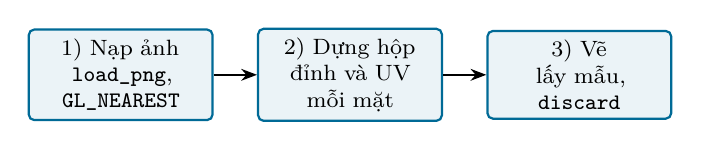
\begin{tikzpicture}[node distance=5.5mm]
\node[pbox] (a) {1) Nạp ảnh \\ \code{load\_png}, \code{GL\_NEAREST}};
\node[pbox,right=of a] (b) {2) Dựng hộp \\ đỉnh và UV mỗi mặt};
\node[pbox,right=of b] (c) {3) Vẽ \\ lấy mẫu, \code{discard}};
\draw[parr] (a)--(b); \draw[parr] (b)--(c);
\end{tikzpicture}
\caption{Ba bước vẽ skin.}
\label{fig:skinflow}
\end{figure}

\textbf{1) Dựng hộp.} Hộp có tâm, kích thước $(w,h,d)$ và độ phồng nhỏ $\delta$. Mỗi góc trong tám góc là tâm dịch đi một nửa mỗi kích thước, cộng thêm $\delta$, theo một hướng.
Mỗi hộp được dựng hai lần: lớp nền ($\delta=0$) và lớp áo ($\delta=0{,}25$ cho thân, tay, chân; $0{,}5$ cho mũ). Lớp áo to hơn một chút nên nằm ngay ngoài lớp nền và không dính vào nó.

\par\noindent\fcolorbox{red}{white}{\footnotesize\textbf{Mã nguồn: Listing~\ref{lst:boxcorner} (Phụ lục~\ref{app:code}).}}\par\vspace{3pt}

\textbf{2) Chọn ô trên ảnh.} Hộp có gốc $(o_x,o_y)$ trên skin, và Hình~\ref{fig:skincross} cho thấy sáu mặt của nó nằm ở đâu. Ví dụ đầu có gốc $(0,0)$ và $w=h=d=8$, nên mặt trước (khuôn mặt) là ô $(8,8,8,8)$. Bốn góc của mặt nhận tọa độ UV của bốn góc ô đó trên ảnh (vị trí pixel chia cho 64). Thứ tự bốn góc của ô phải khớp với thứ tự bốn đỉnh của mặt. Nếu lệch thì ảnh bị lật hoặc xoay.

\par\noindent\fcolorbox{red}{white}{\footnotesize\textbf{Mã nguồn: Listing~\ref{lst:skinuv} (Phụ lục~\ref{app:code}).}}\par\vspace{3pt}

\begin{figure}[H]
\centering
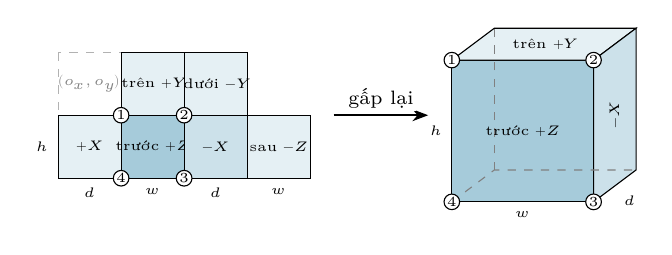
\begin{tikzpicture}[font=\tiny]
% hình chữ thập trên ảnh skin (gốc (o_x,o_y) ở góc trên trái)
\begin{scope}[x=0.4cm,y=-0.4cm]
\draw[dashed,gray!60] (0,0) rectangle (2,2);
\node[gray] at (1,1) {$(o_x,o_y)$};
\draw[fill=linkblue!10] (2,0) rectangle (4,2) node[midway]{trên $+Y$};
\draw[fill=linkblue!10] (4,0) rectangle (6,2) node[midway]{dưới $-Y$};
\draw[fill=linkblue!10] (0,2) rectangle (2,4) node[midway]{$+X$};
\draw[fill=linkblue!35] (2,2) rectangle (4,4) node[midway]{trước $+Z$};
\draw[fill=linkblue!20] (4,2) rectangle (6,4) node[midway]{$-X$};
\draw[fill=linkblue!10] (6,2) rectangle (8,4) node[midway]{sau $-Z$};
\foreach \p/\n in {{2,2}/1,{4,2}/2,{4,4}/3,{2,4}/4}
  \node[circle,fill=white,draw,inner sep=0.3pt] at (\p) {\n};
\node[below] at (1,4) {$d$}; \node[below] at (3,4) {$w$};
\node[below] at (5,4) {$d$}; \node[below] at (7,4) {$w$};
\node[left] at (0,3) {$h$};
\end{scope}
\draw[parr] (3.5,-0.8) -- node[plab,above=1pt]{gấp lại} (4.7,-0.8);
% hộp 3D tương ứng (phép chiếu xiên)
\begin{scope}[shift={(5.0,-1.9)},x=0.9cm,y=0.9cm]
\draw[fill=linkblue!35] (0,0) rectangle (2,2);
\draw[fill=linkblue!10] (0,2) -- (2,2) -- (2.6,2.45) -- (0.6,2.45) -- cycle;
\draw[fill=linkblue!20] (2,0) -- (2.6,0.45) -- (2.6,2.45) -- (2,2) -- cycle;
\draw[dashed,gray] (0,0) -- (0.6,0.45) -- (2.6,0.45); \draw[dashed,gray] (0.6,0.45) -- (0.6,2.45);
\node at (1,1) {trước $+Z$};
\node at (1.3,2.22) {trên $+Y$};
\node[rotate=90] at (2.3,1.22) {$-X$};
\foreach \p/\n in {{0,2}/1,{2,2}/2,{2,0}/3,{0,0}/4}
  \node[circle,fill=white,draw,inner sep=0.3pt] at (\p) {\n};
\node[below] at (1,0) {$w$}; \node[left] at (0,1) {$h$};
\node[below right] at (2.3,0.22) {$d$};
\end{scope}
\end{tikzpicture}
\caption{Hộp 3D và hình chữ thập của nó. Mặt $+Z$ ($w\times h$) có ô $(o_x{+}d,\,o_y{+}d,\,w,\,h)$, mặt $+Y$ có ô $(o_x{+}d,\,o_y,\,w,\,d)$. Bốn góc 1, 2, 3, 4 của mỗi mặt khớp với bốn góc 1, 2, 3, 4 của ô của nó.}
\label{fig:skincross}
\end{figure}

\textbf{3) Vẽ.} Skin được nạp bằng hàm \code{load\_png} em tự viết. Bộ lọc \code{GL\_NEAREST} giữ cho pixel sắc nét ($\lfloor 64u\rfloor,\lfloor 64v\rfloor$). Fragment shader bỏ pixel có $\alpha<0{,}5$, nên chỗ trong suốt của lớp áo để lộ lớp nền. Màu cuối là màu texel cộng thêm một ánh sáng đơn giản. Mỗi hộp được vẽ với ma trận model riêng, nên tay và chân xoay độc lập quanh khớp.

\begin{figure}[H]
\centering

\includegraphics[width=0.45\columnwidth]{figures/skinzom.png}
\caption{Skin $64\times64$ của nhân vật. Mỗi hộp (đầu, thân, tay, chân) có một hình chữ thập cho lớp nền và một hình cho lớp áo (mũ, áo, tay áo).}
\label{fig:skin}
\end{figure}

Dán skin (Hình~\ref{fig:skin}) lên hình chữ thập của các hộp (Hình~\ref{fig:skincross}) cho ra nhân vật có texture ở Hình~\ref{fig:t3result}.

\begin{figure}[H]
\centering
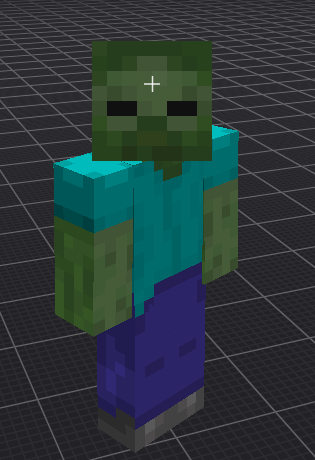
\includegraphics[width=0.4\columnwidth]{figures/t3.png}
\caption{Kết quả ánh xạ texture: skin ở Hình~\ref{fig:skin} được dán lên các hộp ở Hình~\ref{fig:skincross}.}
\label{fig:t3result}
\end{figure}

%====================================================================
\section{T4: Ánh sáng và bóng đổ}
\label{chap:t4}
%====================================================================
Màu cuối của một gaussian được tạo qua bốn phần.
\begin{itemize}\itemsep0pt
\item Phần 1, màu phụ thuộc hướng nhìn: đọc màu gốc từ các hệ số SH.
\item Phần 2, chiếu sáng Phong: cộng ánh sáng môi trường, khuếch tán và phản chiếu.
\item Phần 3, mặt trời: di chuyển mặt trời và đổi màu trời theo giờ.
\item Phần 4, bóng đổ: kiểm tra từng gaussian với shadow map.
\end{itemize}

\subsection{Phần 1: Màu phụ thuộc hướng nhìn}
\label{sec:sh}
Màu của một gaussian thay đổi theo hướng nhìn $\mathbf{d}$. 3DGS lưu sự phụ thuộc này bằng các hệ số điều hòa cầu (SH) \cite{kerbl2023gaussian}:
\begin{equation}
\mathbf{c}(\mathbf{d})=\operatorname{clip}\!\Big(\mathbf{c}_0+\sum_{k=1}^{K}Y_k(\mathbf{d})\,\mathbf{h}_k,\,0,\,1\Big).
\label{eq:sh}
\end{equation}
Ở đây $\mathbf{c}_0$ là màu cơ bản, $\mathbf{h}_k$ là các hệ số trong file và $Y_k$ là các hàm cơ sở. Các hệ số nằm trong không gian file, nên shader quay hướng nhìn về không gian đó: $\mathbf{d}=\operatorname{norm}\!\big(\mathbf{A}^{\top}(\mathbf{p}_w-\mathbf{e})\big)$. Nhờ vậy không phải quay các hệ số trong mỗi khung hình. Hình~\ref{fig:sh} minh họa ý tưởng cho bậc 0 đến 2. Mỗi hàm cơ sở là một mẫu hình trên mặt cầu, và tổng có trọng số của chúng cho một màu ứng với mỗi hướng nhìn.

\par\noindent\fcolorbox{red}{white}{\footnotesize\textbf{Mã nguồn: Listing~\ref{lst:sh} (Phụ lục~\ref{app:code}).}}\par\vspace{3pt}

\begin{figure}[H]
\centering
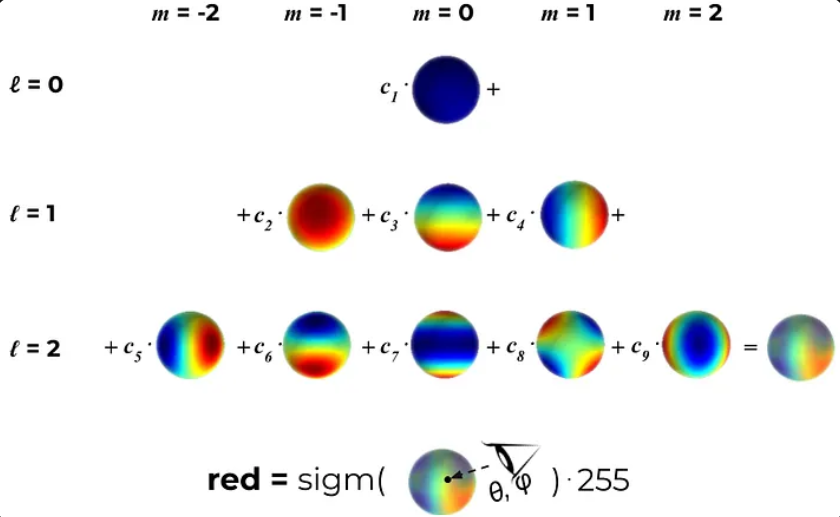
\includegraphics[width=0.8\columnwidth]{figures/1 (1).png}
\caption{Điều hòa cầu đến bậc 2. Chín hàm cơ sở được nhân với các hệ số $c_1..c_9$ rồi cộng lại. Màu được đọc tại hướng nhìn $(\theta,\varphi)$.}
\label{fig:sh}
\end{figure}

\subsection{Phần 2: Chiếu sáng Phong}
Ánh sáng được tính một lần cho mỗi gaussian. Pháp tuyến $\mathbf{n}$ là trục ngắn nhất của ellipsoid, lật về phía camera. Màu cuối theo mô hình Phong \cite{phong1975}, gồm ba phần (Hình~\ref{fig:phong}). Gọi $\mathbf{c}$ là màu của gaussian.

\textbf{Ambient.} Ánh sáng môi trường $\mathbf{L}_a$ chiếu đều lên mọi gaussian:
\begin{equation}
\mathbf{I}_a=\mathbf{c}\,\mathbf{L}_a.
\label{eq:phong-a}
\end{equation}

\textbf{Diffuse.} Mặt hướng về đèn thì sáng hơn. Với đèn $j$, $\mathbf{L}_j$ là màu và $\mathbf{l}_j$ là hướng về đèn:
\begin{equation}
\begin{aligned}
\mathbf{I}_d&=\mathbf{c}\sum_j \mathbf{L}_j\,w(\mathbf{n},\mathbf{l}_j)\,S_j,\\
w(\mathbf{n},\mathbf{l})&=\operatorname{clip}\!\Big(\frac{\mathbf{n}\!\cdot\!\mathbf{l}+0{,}35}{1{,}35},0,1\Big).
\end{aligned}
\label{eq:phong-d}
\end{equation}
$w$ là $\mathbf{n}\!\cdot\!\mathbf{l}$ đã làm mềm. Phải làm mềm vì pháp tuyến ước lượng khá nhiễu.

\textbf{Specular.} Điểm sáng bóng hiện ra khi tia phản xạ $\mathbf{r}_j$ gần với hướng $\mathbf{v}$ về camera:
\begin{equation}
\mathbf{I}_s=k_s\sum_{j}\mathbf{L}_j\,(\mathbf{r}_j\!\cdot\!\mathbf{v})_{+}^{m}\,S_j.
\label{eq:phong-s}
\end{equation}
Ở đây $k_s$ là cường độ specular và $m$ là độ bóng. Phần này không dùng màu $\mathbf{c}$, và bằng 0 khi $\mathbf{n}\!\cdot\!\mathbf{l}_j\le0$.

\textbf{Tổng.} Màu cuối là tổng của ba phần:
\begin{equation}
\mathbf{c}_{out}=\mathbf{I}_a+\mathbf{I}_d+\mathbf{I}_s.
\label{eq:phong-wrap}
\end{equation}
$S_j$ là hệ số bóng đổ với mặt trời, và là độ suy giảm theo khoảng cách với đèn điểm. Cảnh có một mặt trời và tối đa 8 đèn điểm. Đèn điểm không đổ bóng.

\par\noindent\fcolorbox{red}{white}{\footnotesize\textbf{Mã nguồn: Listing~\ref{lst:phong} (Phụ lục~\ref{app:code}).}}\par\vspace{3pt}

\begin{figure}[H]
\centering
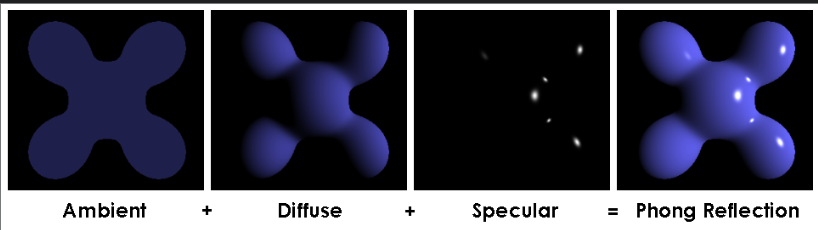
\includegraphics[width=\columnwidth]{figures/1 (2).png}
\caption{Mô hình Phong \cite{phong1975}: phần ambient, diffuse và specular, và tổng của chúng.}
\label{fig:phong}
\end{figure}

\subsection{Phần 3: Mặt trời}
Hướng mặt trời tính từ giờ $h$ trong ngày. Mặt trời mọc lúc 6 giờ, cao nhất lúc 12 giờ và lặn lúc 18 giờ. Màu trời và ánh sáng môi trường đổi dần giữa ngày và đêm, và hơi ngả cam lúc hoàng hôn (Hình~\ref{fig:t4}).

\subsection{Phần 4: Bóng đổ}
Chương trình vẽ tâm các gaussian đặc thành điểm vào một depth map $2048^2$ nhìn từ mặt trời \cite{williams1978}. Sau đó mỗi gaussian được chiếu vào map này để so độ sâu của nó với độ sâu đã lưu. Nếu có vật gần mặt trời hơn, gaussian nằm trong bóng. Lấy trung bình $3\times3$ mẫu sẽ làm mềm cạnh bóng (PCF \cite{reeves1987}):
\begin{equation}
S=\frac19\sum_{i,j=-1}^{1}\big[\,z_s-b\le D_s(u_s+i\tau,\,v_s+j\tau)\,\big].
\label{eq:pcf}
\end{equation}
Ở đây $(u_s,v_s,z_s)$ là tọa độ của gaussian trong map, $D_s$ là độ sâu đã lưu, $\tau$ là bước texel và $b$ là bias. Bias ngăn gaussian tự đổ bóng lên chính nó.

\par\noindent\fcolorbox{red}{white}{\footnotesize\textbf{Mã nguồn: Listing~\ref{lst:pcf} (Phụ lục~\ref{app:code}).}}\par\vspace{3pt}

\par\noindent\fcolorbox{red}{white}{\footnotesize\textbf{Mã nguồn: Listing~\ref{lst:shadowsetup} (Phụ lục~\ref{app:code}).}}\par\vspace{3pt}

%====================================================================
\section{T5: Hoạt họa và mô phỏng}
\label{chap:t5}
%====================================================================
Mọi chuyển động đều nhân với thời gian khung hình $\Delta t$, nên tốc độ ít phụ thuộc vào máy. Ba phần dưới đây chạy theo đúng thứ tự này trong một khung hình.
\begin{itemize}\itemsep0pt
\item Phần 1, chu kỳ ngày đêm: chạy đồng hồ và di chuyển mặt trời.
\item Phần 2, va chạm voxel: biến các gaussian thành voxel đặc.
\item Phần 3, người chơi: đi, nhảy và rơi trên các voxel.
\end{itemize}

\subsection{Phần 1: Chu kỳ ngày đêm}
Chu kỳ là một máy trạng thái có 4 trạng thái: NIGHT $\to$ DAWN $\to$ DAY $\to$ DUSK. Đồng hồ tự chạy. Các trạng thái bắt đầu lúc 5 giờ (DAWN), 7 giờ (DAY), 17 giờ (DUSK) và 19 giờ (NIGHT). Đèn đặt ``bật vào ban đêm'' sẽ bật lúc hoàng hôn và tắt lúc bình minh. Một ngày dài $T_{day}=36$ giây, nên mỗi khung hình giờ tăng $\Delta h = 24\,\Delta t/T_{day}$. Vị trí mặt trời tính theo giờ:
\begin{equation}
\begin{gathered}
\theta=\frac{h-6}{12}\pi,\qquad
\epsilon=65^{\circ}\sin\theta,\
\mathbf{s}=\big(\cos\epsilon\cos\phi,\;\sin\epsilon,\;\cos\epsilon\sin\phi\big),
\end{gathered}
\label{eq:sun}
\end{equation}
trong đó $\phi=\phi_0+\theta-\pi/2$ và $\phi_0$ là góc phương vị của mặt trời. Theo công thức này, mặt trời mọc lúc 6 giờ, cao nhất lúc 12 giờ và lặn lúc 18 giờ. Hệ số ánh sáng ngày là $D=\operatorname{smoothstep}(-0{,}08,\,0{,}3,\,s_y)$. $D$ trộn màu môi trường và màu bầu trời giữa giá trị ban đêm và ban ngày. Bầu trời có thêm sắc cam gần đường chân trời.

\par\noindent\fcolorbox{red}{white}{\footnotesize\textbf{Mã nguồn: Listing~\ref{lst:sun} (Phụ lục~\ref{app:code}).}}\par\vspace{3pt}

\subsection{Phần 2: Va chạm với voxel}
Gaussian không có bề mặt rõ ràng, nên khó tính va chạm trực tiếp. Chương trình chia không gian thành các voxel cạnh $v$, và voxel nào chứa đủ gaussian thì được coi là đặc. Mỗi voxel đặc được lưu thành một số nguyên 64 bit:
\begin{equation}
\mathbf{c} = \left\lfloor \frac{\mathbf{p}-\mathbf{o}}{v} \right\rfloor,
\qquad
\text{key} = (c_x \ll 42)\,|\,(c_z \ll 21)\,|\,c_y.
\label{eq:voxel}
\end{equation}
Các khóa luôn được giữ theo thứ tự tăng dần. Vì $c_y$ nằm ở các bit thấp, các ô cùng một cột đứng liền nhau. Nhờ vậy tìm mặt đất dưới chân chỉ cần một lệnh \code{np.searchsorted}.

\par\noindent\fcolorbox{red}{white}{\footnotesize\textbf{Mã nguồn: Listing~\ref{lst:voxel} (Phụ lục~\ref{app:code}).}}\par\vspace{3pt}

\begin{figure}[H]
\centering
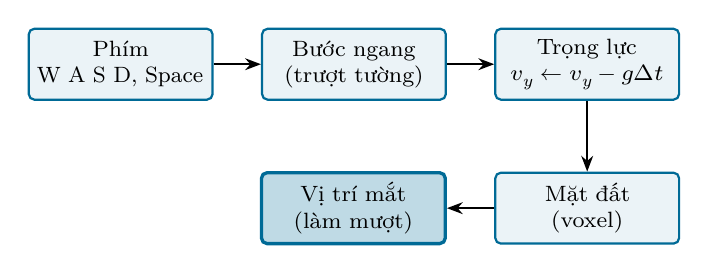
\begin{tikzpicture}[node distance=9mm and 6mm]
  \node[pbox] (key) {Phím\\W A S D, Space};
  \node[pbox,right=of key] (move) {Bước ngang\\(trượt tường)};
  \node[pbox,right=of move] (grav) {Trọng lực\\$v_y\leftarrow v_y-g\Delta t$};
  \node[pbox,below=of grav] (gr) {Mặt đất\\(voxel)};
  \node[pmine,left=of gr] (eye) {Vị trí mắt\\(làm mượt)};
  \draw[parr] (key) -- (move);
  \draw[parr] (move) -- (grav);
  \draw[parr] (grav) -- (gr);
  \draw[parr] (gr) -- (eye);
\end{tikzpicture}
\caption{Một khung hình của chế độ đi bộ.}
\label{fig:t5}
\end{figure}

\subsection{Phần 3: Người chơi}
Hình~\ref{fig:t5} tóm tắt một khung hình. Người chơi là một hình trụ, trượt dọc theo tường, leo được bậc thấp và nhảy được.

\textbf{Trọng lực.} Khi người chơi không đứng trên đất, chương trình tích phân theo Euler:
\begin{equation}
v_y \leftarrow v_y - g\,\Delta t,
\qquad
y \leftarrow y + v_y\,\Delta t.
\label{eq:euler}
\end{equation}
\textbf{Tỉ lệ và cú nhảy.} Cảnh 3DGS không có đơn vị cố định, nên mọi kích thước và tốc độ đều tỉ lệ theo chiều cao người chơi $H$. Các hằng số là: cạnh voxel $v=H/8$, bán kính người chơi $0{,}14H$, chiều cao bậc $0{,}35H$, trọng lực $g=12H$, tốc độ đi $2{,}5H$ mỗi giây (chạy nhanh $\times1{,}7$, đi chậm $\times0{,}4$). Cú nhảy đạt độ cao $0{,}75H$, nên vận tốc lúc bật lên là
\begin{equation}
v_0=\sqrt{2\,g\,(0{,}75H)}.
\label{eq:jump}
\end{equation}
\textbf{Làm mượt mắt.} Khi người chơi đứng trên đất, độ cao mắt được làm mượt để bề mặt gaussian gồ ghề không làm rung camera.

\par\noindent\fcolorbox{red}{white}{\footnotesize\textbf{Mã nguồn: Listing~\ref{lst:jump} (Phụ lục~\ref{app:code}).}}\par\vspace{3pt}

%====================================================================
\section{T6: Tương tác và giao diện}
\label{chap:t6}
%====================================================================
Tương tác có bốn phần, từ đầu vào đến màn hình.
\begin{itemize}\itemsep0pt
\item Phần 1, xử lý sự kiện: quyết định ai nhận mỗi sự kiện chuột hoặc phím.
\item Phần 2, chọn bằng cọ: chọn gaussian bằng cách tô lên màn hình.
\item Phần 3, xóa mềm và hoàn tác: xóa vùng chọn và khôi phục lại.
\item Phần 4, giao diện: bảng điều khiển, HUD và phím tắt.
\end{itemize}

\subsection{Phần 1: Xử lý sự kiện}
Sự kiện chuột và bàn phím đến ImGui trước. Sự kiện nào ImGui không dùng thì đi tiếp đến camera, cọ chọn và các phím tắt.

\subsection{Phần 2: Chọn bằng cọ}
Nhấn \code{B} để bật cọ. Tô lên màn hình sẽ chọn các gaussian, và chúng chuyển sang màu vàng. Để kiểm tra, tâm mỗi gaussian được chiếu thành pixel $\mathbf{p}$ (Mục~\ref{sec:cam}).

\textbf{Kiểm tra capsule.} Một nét vẽ từ $\mathbf{a}$ đến $\mathbf{b}$ là một capsule bán kính $r$. Gaussian được chọn nếu
\begin{equation}
\lVert\mathbf{p}-\mathbf{a}-\tau(\mathbf{b}-\mathbf{a})\rVert\le r,\quad \tau=\operatorname{clip}\tfrac{(\mathbf{p}-\mathbf{a})\cdot(\mathbf{b}-\mathbf{a})}{\lVert\mathbf{b}-\mathbf{a}\rVert^2}\in[0,1].
\label{eq:capsule}
\end{equation}
Nói cách khác, khoảng cách từ $\mathbf{p}$ đến đoạn $\mathbf{ab}$ không quá $r$.

\par\noindent\fcolorbox{red}{white}{\footnotesize\textbf{Mã nguồn: Listing~\ref{lst:capsule} (Phụ lục~\ref{app:code}).}}\par\vspace{3pt}
 

\textbf{Tính chất.} Cọ chỉ xét tâm gaussian và bỏ qua độ sâu, nên nó chọn xuyên qua cảnh, giống SuperSplat \cite{supersplat}. Để nhanh, cọ loại cả khối 1024 gaussian khi hộp bao của khối nằm ngoài nét vẽ.

\subsection{Phần 3: Xóa mềm và hoàn tác}
Mỗi gaussian có một byte trạng thái trên GPU với hai bit: \emph{đã chọn} và \emph{đã xóa}. Lệnh \code{Delete} chỉ bật bit ``đã xóa''. Shader sẽ bỏ qua các gaussian này, còn dữ liệu gốc không đổi. Mỗi lần xóa là một lệnh trong \code{History} (mẫu Command \cite{gamma1994design}, tối đa 20 bước), và \code{Ctrl+Z} hoàn tác lệnh cuối.

\par\noindent\fcolorbox{red}{white}{\footnotesize\textbf{Mã nguồn: Listing~\ref{lst:history} (Phụ lục~\ref{app:code}).}}\par\vspace{3pt}

\subsection{Phần 4: Giao diện}
Bảng ImGui bên trái điều khiển layer, phép biến đổi, vùng chọn, chế độ camera và ánh sáng. HUD hiển thị tâm ngắm, đồng hồ, vị trí và vòng tròn cọ. Bảng~\ref{tab:keys} liệt kê các phím chính.
\begin{table}[H]
\centering
\caption{Các phím điều khiển chính.}
\label{tab:keys}
\footnotesize
\begin{tabular}{@{}p{3.1cm}p{4.6cm}@{}}
\toprule
Phím / chuột & Chức năng \\
\midrule
Kéo chuột trái / giữa & Xoay quanh / pan \\
Kéo chuột phải + \code{WASD} & Nhìn quanh, bay (\code{Ctrl} = nhanh) \\
\code{M}, \code{F5}, \code{C}, \code{V} & Bay/đi bộ; góc nhìn thứ ba; ngồi; vẫy tay \\
\code{F}, \code{G} & Xem toàn cảnh; hiện/ẩn lưới \\
\code{B}, \code{[}, \code{]} & Cọ chọn; cỡ cọ \\
\code{Delete}, \code{Ctrl+Z} & Xóa / hoàn tác \\
\code{Ctrl+O/I/S} & Mở / thêm layer / lưu \\
\bottomrule
\end{tabular}
\end{table}

%====================================================================
\section{Hạn chế và hướng phát triển}
\label{chap:future}
%====================================================================
\subsection{Hạn chế}
\begin{itemize}\itemsep0pt
\item Tốc độ phụ thuộc CPU. Độ sâu được sắp xếp bằng NumPy trong một luồng nền (Mục~\ref{sec:blend}). Khi camera quay nhanh, hình có thể nhấp nháy, và cảnh lớn phải giới hạn số gaussian được vẽ (LOD).
\item Hình học chỉ là xấp xỉ. Gaussian không có bề mặt thật, nên cọ chọn, va chạm, pháp tuyến và bóng đều dựa vào tâm gaussian. Hệ quả là cọ chọn cả vật bị che, va chạm có thể thủng lỗ và ánh sáng còn thô.
\end{itemize}

\subsection{Hướng phát triển}
\begin{itemize}\itemsep0pt
\item Mô phỏng. Bản đồ voxel và phần vật lý có sẵn có thể dùng để mô phỏng chuyển động trong cảnh quay từ đời thực, ví dụ thử đường đi của người, robot hay xe. Việc này cần va chạm chính xác hơn và thêm các vật thể động.
\item Game. Cảnh 3DGS có thể thành một màn chơi có nhân vật máy, vật phẩm và nhiệm vụ, vẫn giữ chu kỳ ngày đêm và đèn. Cảnh đã làm sạch có thể xuất sang game engine như Unity hoặc Unreal.
\end{itemize}

%====================================================================
\section{Tuyên bố sử dụng AI}
\label{chap:ai}
%====================================================================
Theo quy định của môn học, sinh viên được dùng công cụ AI (ChatGPT, Gemini) để học khái niệm, gỡ lỗi và cải thiện mã nguồn. Trong đồ án này, em đã dùng ChatGPT và Gemini cho hai việc:
\begin{itemize}\itemsep0pt
\item Học khái niệm: giải thích 3D Gaussian Splatting, EWA, điều hòa cầu, bản đồ bóng và các kỹ thuật đồ họa liên quan.
\item Gỡ lỗi và cải thiện mã: tìm lỗi, gợi ý cách viết gọn và nhanh hơn cho chương trình.
\end{itemize}
Em đã đọc, kiểm tra và chạy thử nội dung do AI gợi ý, và chịu trách nhiệm về toàn bộ mã nguồn và báo cáo này.

%====================================================================
\section{Kết luận}
\label{chap:end}
%====================================================================
Splat Editor đọc, hiển thị, chỉnh sửa và lưu được file 3DGS, và dùng đủ sáu nhóm kỹ thuật của môn học. Bảng~\ref{tab:src} liệt kê các file mã nguồn của từng phần.

\begin{table}[H]
\centering
\caption{Các file mã nguồn chính (trong \code{splat\_editor/}).}
\label{tab:src}
\footnotesize
\begin{tabular}{@{}p{2.2cm}>{\raggedright\arraybackslash}p{5.5cm}@{}}
\toprule
Phần & File \\
\midrule
Đọc/ghi PLY & \mbox{\code{io/ply.py}}, \mbox{\code{io/codec.py}} \\
Hiển thị gaussian & \mbox{\code{render/splat\_renderer.py}}, \mbox{\code{render/sorter.py}}, \mbox{\code{render/shaders/splat\_prep.vert}} \\
T1 & \mbox{\code{core/layer.py}}, \mbox{\code{core/transform.py}}, \mbox{\code{core/avatar\_pose.py}} \\
T2 & \mbox{\code{core/math3d.py}}, \mbox{\code{render/camera.py}} \\
T3 & \mbox{\code{render/avatar\_renderer.py}} \\
T4 & \mbox{\code{core/sh.py}}, \mbox{\code{core/lighting.py}}, \mbox{\code{render/shaders/shadow.vert}} \\
T5 & \mbox{\code{core/physics.py}}, \mbox{\code{core/avatar\_pose.py}} \\
T6 & \mbox{\code{editor/brush.py}}, \mbox{\code{core/history.py}}, \mbox{\code{ui/}} \\
\bottomrule
\end{tabular}
\end{table}

\begin{thebibliography}{99}\footnotesize\itemsep0pt\parskip0pt
\bibitem{schonberger2016colmap} J.~L.~Sch{\"o}nberger, J.-M.~Frahm, Structure-from-motion revisited, in: CVPR, 2016, pp.~4104--4113.
\bibitem{kerbl2023gaussian} B.~Kerbl, G.~Kopanas, T.~Leimk{\"u}hler, G.~Drettakis, 3D Gaussian splatting for real-time radiance field rendering, ACM Trans. Graph. 42(4) (2023) 139.
\bibitem{supersplat} PlayCanvas, SuperSplat: an open-source 3D Gaussian Splat editor, \url{https://github.com/playcanvas/supersplat}.
\bibitem{zwicker2002ewa} M.~Zwicker, H.~Pfister, J.~van Baar, M.~Gross, EWA splatting, IEEE Trans. Vis. Comput. Graph. 8(3) (2002) 223--238.
\bibitem{phong1975} B.~T.~Phong, Illumination for computer generated pictures, Commun. ACM 18(6) (1975) 311--317.
\bibitem{williams1978} L.~Williams, Casting curved shadows on curved surfaces, in: SIGGRAPH, 1978, pp.~270--274.
\bibitem{reeves1987} W.~T.~Reeves, D.~H.~Salesin, R.~L.~Cook, Rendering antialiased shadows with depth maps, in: SIGGRAPH, 1987, pp.~283--291.
\bibitem{gamma1994design} E.~Gamma, R.~Helm, R.~Johnson, J.~Vlissides, Design Patterns: Elements of Reusable Object-Oriented Software, Addison-Wesley, 1994.
\end{thebibliography}


%====================================================================
% APPENDIX: all code listings, large font, one column
%====================================================================
\clearpage
\onecolumn
\appendix
\lstset{basicstyle=\ttfamily\fontsize{7.2}{8.6}\selectfont,numbers=left,numberstyle=\tiny\color{gray},
  numbersep=6pt,xleftmargin=16pt,framexleftmargin=14pt,frame=single,rulecolor=\color{gray!60},
  backgroundcolor=\color{gray!5},framerule=0.5pt,aboveskip=6pt,belowskip=10pt,
  breaklines=true,breakindent=0pt,captionpos=t}
\captionsetup[lstlisting]{skip=4pt,font={small,bf},labelfont=bf}
\section{Mã nguồn các đoạn code}
\label{app:code}
Mọi đoạn code đều được trích từ chương trình. Phần nội dung chính dẫn tới từng đoạn bằng số thứ tự.

\subsection{Giới thiệu và lý thuyết gaussian}
\begin{minipage}{\linewidth}
\begin{lstlisting}[language=Python,caption={\code{io/codec.py}, \code{SplatCodec.\_decode\_block}: giải mã giá trị thô của file PLY},label={lst:decode}]
@staticmethod
def _decode_block(data, names, dtype):
    def col(name):
        """Lấy một cột của file PLY dưới dạng float32."""
        return data[name].astype(np.float32)

    n = len(data['x'])
    positions = np.stack([col('x'), col('y'), col('z')], axis=1)

    if 'f_dc_0' in names:
        colors = 0.5 + SH_C0 * np.stack([col('f_dc_0'), col('f_dc_1'), col('f_dc_2')], axis=1)
    elif 'red' in names:
        colors = np.stack([col('red'), col('green'), col('blue')], axis=1)
        if dtype['red'].kind in 'ui':
            colors /= 255.0
    else:
        colors = np.full((n, 3), 0.7, np.float32)

    alphas = 1.0 / (1.0 + np.exp(-col('opacity'))) if 'opacity' in names else np.ones(n, np.float32)

    if 'scale_0' in names:
        scales = np.exp(np.stack([col('scale_0'), col('scale_1'), col('scale_2')], axis=1))
    else:
        scales = np.ones((n, 3), np.float32)

    identity_quat = np.float32([1, 0, 0, 0])
    if 'rot_0' in names:
        q = np.stack([col('rot_0'), col('rot_1'), col('rot_2'), col('rot_3')], axis=1)
        length = np.linalg.norm(q, axis=1, keepdims=True)
        q = np.where(length > 0, q / np.maximum(length, 1e-12), identity_quat)
    else:
        q = np.tile(identity_quat, (n, 1))
    return positions, colors, alphas, scales, q
\end{lstlisting}
\end{minipage}
\par\vspace{4pt}

\begin{minipage}{\linewidth}
\begin{lstlisting}[language=GLSL,caption={\code{render/shaders/splat\_prep.vert}, \code{quatToMat3}, \code{covariance3D}: dựng $\Sigma=\mathbf{R}\mathbf{S}\mathbf{S}^{\top}\mathbf{R}^{\top}$},label={lst:cov3d}]
mat3 quatToMat3(vec4 q) {
    float w = q.x, x = q.y, y = q.z, z = q.w;
    return mat3(1.0 - 2.0 * (y * y + z * z), 2.0 * (x * y + w * z), 2.0 * (x * z - w * y),
                2.0 * (x * y - w * z), 1.0 - 2.0 * (x * x + z * z), 2.0 * (y * z + w * x),
                2.0 * (x * z + w * y), 2.0 * (y * z - w * x), 1.0 - 2.0 * (x * x + y * y));
}

mat3 covariance3D(mat3 R, vec3 scale) {
    mat3 M = R * mat3(scale.x, 0.0, 0.0, 0.0, scale.y, 0.0, 0.0, 0.0, scale.z);
    return M * transpose(M);
}
\end{lstlisting}
\end{minipage}
\par\vspace{4pt}


\subsection{T1: Phép biến đổi và mô hình phân cấp}
\begin{minipage}{\linewidth}
\begin{lstlisting}[language=Python,caption={\code{core/math3d.py} và \code{core/layer.py}: ma trận $\mathbf{M}$ của layer},label={lst:world}]
def euler_to_matrix(degrees):
    x, y, z = np.radians(degrees)
    cx, sx, cy, sy, cz, sz = math.cos(x), math.sin(x), math.cos(y), math.sin(y), math.cos(z), math.sin(z)
    rx = np.array([[1, 0, 0], [0, cx, -sx], [0, sx, cx]])
    ry = np.array([[cy, 0, sy], [0, 1, 0], [-sy, 0, cy]])
    rz = np.array([[cz, -sz, 0], [sz, cz, 0], [0, 0, 1]])
    return rz @ ry @ rx

def world_transform(self, flip):
    rot = self.transform.rotation_matrix() @ (FLIP if flip else np.identity(3))
    return rot, self.transform.translation(), float(self.transform.scale)

def world_matrix(self, flip):
    rot, t, s = self.world_transform(flip)
    m = np.identity(4)
    m[:3, :3] = s * rot
    m[:3, 3] = t
    return m
\end{lstlisting}
\end{minipage}
\par\vspace{4pt}

\begin{minipage}{\linewidth}
\begin{lstlisting}[language=Python,caption={\code{core/transform.py}, \code{Transform.rotate\_about}},label={lst:pivot}]
def rotate_about(self, delta, pivot):
    pivot = np.asarray(pivot, float)
    self.rotation = matrix_to_euler(delta @ self.rotation_matrix())
    self.position = list(delta @ (self.translation() - pivot) + pivot)
\end{lstlisting}
\end{minipage}
\par\vspace{4pt}


\subsection{T2: Camera và phép chiếu}
\begin{minipage}{\linewidth}
\begin{lstlisting}[language=Python,caption={\code{core/math3d.py}, \code{look\_at}: ma trận nhìn $\mathbf{V}$},label={lst:lookat}]
def look_at(eye, target, up):
    forward = target - eye
    forward /= np.linalg.norm(forward)
    right = np.cross(forward, up)
    right /= np.linalg.norm(right)
    true_up = np.cross(right, forward)

    m = np.identity(4, np.float32)
    m[0, :3] = right
    m[1, :3] = true_up
    m[2, :3] = -forward
    m[:3, 3] = -m[:3, :3] @ eye
    return m
\end{lstlisting}
\end{minipage}
\par\vspace{4pt}

\begin{minipage}{\linewidth}
\begin{lstlisting}[language=Python,caption={\code{core/math3d.py}, \code{perspective}: ma trận chiếu $\mathbf{P}$},label={lst:persp}]
def perspective(fov_y_deg, aspect, near, far):
    zoom = 1.0 / math.tan(math.radians(fov_y_deg) / 2)
    m = np.zeros((4, 4), np.float32)
    m[0, 0] = zoom / aspect
    m[1, 1] = zoom
    m[2, 2] = (far + near) / (near - far)
    m[2, 3] = 2 * far * near / (near - far)
    m[3, 2] = -1
    return m
\end{lstlisting}
\end{minipage}
\par\vspace{4pt}

\begin{minipage}{\linewidth}
\begin{lstlisting}[language=GLSL,caption={\code{render/shaders/splat\_prep.vert}, \code{projectCovariance}: Jacobian $\mathbf{J}$ và $\Sigma'=\mathbf{J}\mathbf{W}\Sigma\mathbf{W}^{\top}\mathbf{J}^{\top}$},label={lst:ewa}]
mat3 projectCovariance(mat3 sigma, vec3 viewPos, mat3 linear) {
    float vx = viewPos.x, vy = viewPos.y, vz = viewPos.z;
    mat3 J = mat3(uFocal / -vz, 0.0, 0.0,
                  0.0, uFocal / -vz, 0.0,
                  uFocal * vx / (vz * vz), uFocal * vy / (vz * vz), 0.0);
    mat3 T = J * mat3(uModelView) * linear;
    return T * sigma * transpose(T);
}
\end{lstlisting}
\end{minipage}
\par\vspace{4pt}

\begin{minipage}{\linewidth}
\begin{lstlisting}[language=GLSL,caption={\code{render/shaders/splat\_prep.vert}: giá trị riêng và hai trục ellipse},label={lst:eig}]
float a = cov[0][0] + 0.3;
float b = cov[0][1];
float c = cov[1][1] + 0.3;

float mid = 0.5 * (a + c);
float radius = length(vec2(0.5 * (a - c), b));
float lambda1 = mid + radius;
float lambda2 = max(mid - radius, 0.1);
vec2 axis1 = (abs(b) < 1e-6) ? (a >= c ? vec2(1.0, 0.0) : vec2(0.0, 1.0))
                             : normalize(vec2(b, lambda1 - a));
vec2 axis2 = vec2(-axis1.y, axis1.x);

vec2 toNdc = 2.0 / uViewport;
vec2 major = min(extent * sqrt(lambda1), 1024.0) * axis1 * toNdc;
vec2 minor = min(extent * sqrt(lambda2), 1024.0) * axis2 * toNdc;
\end{lstlisting}
\end{minipage}
\par\vspace{4pt}

\begin{minipage}{\linewidth}
\begin{lstlisting}[language=GLSL,caption={\code{render/shaders/splat.frag}, \code{main}: $a=\alpha\,e^{-r^2/2}$},label={lst:frag}]
#version 330 core
in vec4 vColor;
in vec2 vCorner;
out vec4 fragColor;

void main() {
    float r2 = dot(vCorner, vCorner);
    if (r2 > 9.0) discard;
    float alpha = vColor.a * exp(-0.5 * r2);
    if (alpha < 1.0 / 255.0) discard;
    fragColor = vec4(vColor.rgb * alpha, alpha);
}
\end{lstlisting}
\end{minipage}
\par\vspace{4pt}

\begin{minipage}{\linewidth}
\begin{lstlisting}[language=Python,caption={\code{render/splat\_renderer.py}, \code{\_draw\_splats}: phép trộn $\mathbf{C}\leftarrow\mathbf{c}a+(1-a)\mathbf{C}$},label={lst:blend}]
def _draw_splats(self):
    s = self.shader
    s.use()
    GL.glActiveTexture(GL.GL_TEXTURE0)
    GL.glBindTexture(GL.GL_TEXTURE_BUFFER, self.feedback_texture)
    s.set_int('uPrep', 0)
    GL.glDisable(GL.GL_DEPTH_TEST)
    GL.glEnable(GL.GL_BLEND)
    GL.glBlendFunc(GL.GL_ONE, GL.GL_ONE_MINUS_SRC_ALPHA)
    GL.glBindVertexArray(self.vao)
    GL.glDrawArraysInstanced(GL.GL_TRIANGLE_STRIP, 0, 4, self.draw_count)
    GL.glBindVertexArray(0)
\end{lstlisting}
\end{minipage}
\par\vspace{4pt}

\begin{minipage}{\linewidth}
\begin{lstlisting}[language=Python,caption={\code{render/sorter.py}, \code{DepthSorter.sort}: sắp xếp xa $\to$ gần},label={lst:sort}]
@staticmethod
def sort(positions, depth_rows):
    if not isinstance(depth_rows, list):
        depth_rows = [(len(positions), np.asarray(depth_rows, np.float64)[2])]
    depth = np.empty(len(positions), np.float32)
    start = 0
    for count, row in depth_rows:
        row = row.astype(np.float32)
        depth[start:start + count] = positions[start:start + count] @ row[:3] + row[3]
        start += count

    visible = np.flatnonzero(depth < 0)
    depth = depth[visible]
    if len(depth) == 0:
        return np.zeros(0, np.uint32)

    far_z, near_z = float(depth.min()), float(depth.max())
    scale = 65535.0 / (near_z - far_z) if near_z > far_z else 0.0
    depth_key = ((depth - far_z) * scale).astype(np.uint16)

    return visible[np.argsort(depth_key, kind='stable')].astype(np.uint32)
\end{lstlisting}
\end{minipage}
\par\vspace{4pt}

\begin{minipage}{\linewidth}
\begin{lstlisting}[language=Python,caption={\code{editor/brush.py}, \code{BrushTool.\_to\_screen}: từ clip sang pixel},label={lst:pixel}]
@staticmethod
def _to_screen(clip, viewport):
    left, top, width, height = viewport
    x = left + (clip[..., 0] / clip[..., 3] + 1) * 0.5 * width
    y = top + (1 - clip[..., 1] / clip[..., 3]) * 0.5 * height
    return x, y
\end{lstlisting}
\end{minipage}
\par\vspace{4pt}

\begin{minipage}{\linewidth}
\begin{lstlisting}[language=Python,caption={\code{render/camera.py}, \code{OrbitCamera.position}},label={lst:eye}]
def position(self):
    cp = math.cos(self.pitch)
    offset = np.array([cp * math.sin(self.yaw), math.sin(self.pitch), cp * math.cos(self.yaw)])
    return self.target + self.distance * offset
\end{lstlisting}
\end{minipage}
\par\vspace{4pt}

\begin{minipage}{\linewidth}
\begin{lstlisting}[language=Python,caption={\code{render/camera.py}, \code{OrbitCamera.fly}},label={lst:fly}]
def fly(self, forward, right, up, dt, sprint=False):
    s, c = math.sin(self.yaw), math.cos(self.yaw)
    direction = forward * np.array([-s, 0.0, -c]) + right * np.array([c, 0.0, -s])
    length = np.linalg.norm(direction)
    if length > 0:
        direction /= length
    direction[1] = up
    wanted = direction * self.fly_speed * (self.SPRINT_FACTOR if sprint else 1.0)
    self.velocity += (wanted - self.velocity) * min(self.FLY_ACCEL * dt, 1.0)
    if not wanted.any() and np.linalg.norm(self.velocity) < 1e-3 * self.fly_speed:
        self.velocity[:] = 0
    self.target += self.velocity * dt
\end{lstlisting}
\end{minipage}
\par\vspace{4pt}


\subsection{T3: Ánh xạ texture}
\begin{minipage}{\linewidth}
\begin{lstlisting}[language=Python,caption={\code{render/avatar\_renderer.py}, \code{\_box}: góc $\mathbf{p}$ của mặt},label={lst:boxcorner}]
def _box(ox, oy, centre, size, inflate):
    (cx, cy, cz), (w, h, d) = centre, size
    hx, hy, hz = w / 2 + inflate, h / 2 + inflate, d / 2 + inflate
    vertices = []
    for face in range(6):
        rx, ry, rw, rh = _uv_region(face, ox, oy, w, h, d)
        uvs = ((rx, ry), (rx + rw, ry), (rx + rw, ry + rh), (rx, ry + rh))
        for (sx, sy, sz), (u, v) in zip(_FACES[face], uvs):
            vertices.append((cx + sx * hx, cy + sy * hy, cz + sz * hz, *_NORMALS[face], u / SKIN_SIZE, v / SKIN_SIZE))
    return vertices
\end{lstlisting}
\end{minipage}
\par\vspace{4pt}

\begin{minipage}{\linewidth}
\begin{lstlisting}[language=Python,caption={\code{render/avatar\_renderer.py}, \code{\_uv\_region}: ô skin của mặt và UV},label={lst:skinuv}]
def _uv_region(face, ox, oy, w, h, d):
    return ((ox + d, oy + d, w, h),
            (ox + 2 * d + w, oy + d, w, h),
            (ox, oy + d, d, h),
            (ox + d + w, oy + d, d, h),
            (ox + d, oy, w, d),
            (ox + d + w, oy, w, d))[face]
\end{lstlisting}
\end{minipage}
\par\vspace{4pt}


\subsection{T4: Ánh sáng và bóng đổ}
\begin{minipage}{\linewidth}
\begin{lstlisting}[language=GLSL,caption={\code{render/shaders/splat\_prep.vert}, \code{shCoeff}, \code{shColor}: màu SH theo hướng nhìn},label={lst:sh}]
vec3 shCoeff(int splat, int k) {
    return (texelFetch(uSh, splat * uShCount + k).rgb * 255.0 - 128.0) * uShScale;
}

vec3 shColor(int splat, vec3 d) {
    float x = d.x, y = d.y, z = d.z;
    vec3 c = -0.4886025119029199 * y * shCoeff(splat, 0)
           +  0.4886025119029199 * z * shCoeff(splat, 1)
           -  0.4886025119029199 * x * shCoeff(splat, 2);
    if (uShDegree < 2) return c;
    float xx = x * x, yy = y * y, zz = z * z;
    c +=  1.0925484305920792 * x * y * shCoeff(splat, 3)
       -  1.0925484305920792 * y * z * shCoeff(splat, 4)
       + 0.31539156525252005 * (2.0 * zz - xx - yy) * shCoeff(splat, 5)
       -  1.0925484305920792 * x * z * shCoeff(splat, 6)
       +  0.5462742152960396 * (xx - yy) * shCoeff(splat, 7);
    if (uShDegree < 3) return c;
    c += -0.5900435899266435 * y * (3.0 * xx - yy) * shCoeff(splat, 8)
       +   2.890611442640554 * x * y * z * shCoeff(splat, 9)
       -  0.4570457994644658 * y * (4.0 * zz - xx - yy) * shCoeff(splat, 10)
       +  0.3731763325901154 * z * (2.0 * zz - 3.0 * xx - 3.0 * yy) * shCoeff(splat, 11)
       -  0.4570457994644658 * x * (4.0 * zz - xx - yy) * shCoeff(splat, 12)
       +   1.445305721320277 * z * (xx - yy) * shCoeff(splat, 13)
       -  0.5900435899266435 * x * (xx - 3.0 * yy) * shCoeff(splat, 14);
    return c;
}

vec3 color = vec3(rg, ba.x);
if (uShDegree > 0) color += shColor(splat, normalize(transpose(linear) * (center - uCamPos)));
color = clamp(color, 0.0, 1.0);
\end{lstlisting}
\end{minipage}
\par\vspace{4pt}

\begin{minipage}{\linewidth}
\begin{lstlisting}[language=GLSL,caption={\code{render/shaders/splat\_prep.vert}, \code{shade}: Phong},label={lst:phong}]
vec3 shade(vec3 albedo, vec3 worldPos, vec3 n, vec3 v) {
    vec3 diffuse = uAmbient;
    vec3 spec = vec3(0.0);
    if (uSunOn != 0) {
        float ndl = dot(n, uSunDir);
        float shadow = (uShadowOn != 0 && ndl > -0.4) ? shadowFactor(worldPos, n) : 1.0;
        diffuse += uSunColor * clamp((ndl + 0.35) / 1.35, 0.0, 1.0) * shadow;
        if (ndl > 0.0) spec += uSunColor * pow(max(dot(reflect(-uSunDir, n), v), 0.0), uShininess) * shadow;
    }
    for (int i = 0; i < uPointCount; i++) {
        vec3 d = uPointPos[i] - worldPos;
        float dist = length(d);
        vec3 l = d / max(dist, 1e-6);
        float att = clamp(1.0 - (dist * dist) / (uPointRange[i] * uPointRange[i]), 0.0, 1.0);
        att *= att;
        float ndl = dot(n, l);
        diffuse += uPointColor[i] * clamp((ndl + 0.35) / 1.35, 0.0, 1.0) * att;
        if (ndl > 0.0) spec += uPointColor[i] * pow(max(dot(reflect(-l, n), v), 0.0), uShininess) * att;
    }
    return albedo * diffuse + spec * uSpecular;
}
\end{lstlisting}
\end{minipage}
\par\vspace{4pt}

\begin{minipage}{\linewidth}
\begin{lstlisting}[language=GLSL,caption={\code{render/shaders/splat\_prep.vert}, \code{shadowFactor}: PCF $3\times3$},label={lst:pcf}]
float shadowFactor(vec3 worldPos, vec3 n) {
    vec4 lp = uLightVP * vec4(worldPos + n * uShadowTexel * 2.0, 1.0);
    vec3 s = lp.xyz / lp.w * 0.5 + 0.5;
    if (s.x < 0.0 || s.x > 1.0 || s.y < 0.0 || s.y > 1.0 || s.z > 1.0) return 1.0;
    float lit = 0.0;
    for (int i = -1; i <= 1; i++)
        for (int j = -1; j <= 1; j++) {
            float d = textureLod(uShadowMap, s.xy + vec2(i, j) * uShadowInv, 0.0).r;
            lit += (s.z - uShadowBias <= d) ? 1.0 : 0.0;
        }
    return lit / 9.0;
}
\end{lstlisting}
\end{minipage}
\par\vspace{4pt}

\begin{minipage}{\linewidth}
\begin{lstlisting}[language=Python,caption={\code{core/lighting.py}, \code{Lighting.shadow\_setup}: ma trận nhìn từ mặt trời},label={lst:shadowsetup}]
def shadow_setup(self):
    d = self.sun_direction()
    r = self.radius * 1.1
    eye = self.center + d * 2.0 * r
    up = np.array([0.0, 1.0, 0.0]) if abs(d[1]) < 0.99 else np.array([0.0, 0.0, 1.0])
    view = look_at(eye, self.center, up).astype(np.float64)
    proj = orthographic(r, 0.01 * r, 4.0 * r).astype(np.float64)
    texel = 2.0 * r / self.SHADOW_SIZE
    return (proj @ view).astype(np.float32), texel, 3.0 * texel / (3.99 * r)
\end{lstlisting}
\end{minipage}
\par\vspace{4pt}


\subsection{T5: Hoạt họa và mô phỏng}
\begin{minipage}{\linewidth}
\begin{lstlisting}[language=Python,caption={\code{core/lighting.py}: giờ, hướng mặt trời và hệ số ánh sáng ngày},label={lst:sun}]
def sun_direction(self):
    angle = (self.hour - 6.0) / 12.0 * math.pi
    elevation = math.sin(angle) * math.radians(MAX_SUN_ELEVATION)
    azimuth = math.radians(self.sun_azimuth) + (angle - math.pi / 2)
    return np.array([math.cos(elevation) * math.cos(azimuth), math.sin(elevation),
                     math.cos(elevation) * math.sin(azimuth)])

def daylight(self):
    return _smooth(-0.08, 0.3, self.sun_direction()[1])

def update(self, dt):
    if self.animate and self.sun_on:
        hours_per_second = 24.0 / max(self.day_length, 1.0)
        self.hour = (self.hour + dt * hours_per_second) % 24.0
    phase = self.cycle.update(self.hour)
    if phase is not None and self.sun_on:
        self._on_enter(phase)
\end{lstlisting}
\end{minipage}
\par\vspace{4pt}

\begin{minipage}{\linewidth}
\begin{lstlisting}[language=Python,caption={\code{core/physics.py}, \code{CollisionWorld}: khóa voxel và tìm mặt đất},label={lst:voxel}]
def build(self, positions, voxel, min_count=1):
    self.voxel = float(voxel)
    if len(positions) == 0:
        return self
    lo = positions.min(axis=0).astype(np.float64)
    self.origin = lo - self.voxel
    self.min_y, self.max_y = float(lo[1]), float(positions[:, 1].max())
    self.floor_y = float(np.percentile(positions[:, 1], 1.0))
    cells = np.floor((positions - self.origin) / self.voxel).astype(np.int64)
    np.clip(cells, 0, _MASK, out=cells)
    keys = (cells[:, 0] << (2 * _BITS)) | (cells[:, 2] << _BITS) | cells[:, 1]
    if min_count > 1:
        keys, counts = np.unique(keys, return_counts=True)
        keys = keys[counts >= min_count]
    else:
        keys = np.unique(keys)
    self.keys = keys
    self.solid_count = len(keys)
    return self

def _highest(self, x, z, y):
    x, z, y = np.broadcast_arrays(np.asarray(x, float), np.asarray(z, float), np.asarray(y, float))
    cell = np.floor((np.stack([x, y, z], axis=-1) - self.origin) / self.voxel).astype(np.int64)
    ix, iy, iz = cell[..., 0], cell[..., 1], cell[..., 2]
    valid = (ix >= 0) & (ix <= _MASK) & (iz >= 0) & (iz <= _MASK) & (iy >= 0)
    iy = np.minimum(iy, _MASK)
    query = (np.clip(ix, 0, _MASK) << (2 * _BITS)) | (np.clip(iz, 0, _MASK) << _BITS) | iy
    idx = np.searchsorted(self.keys, query, side='right') - 1
    found = self.keys[np.maximum(idx, 0)]
    same = valid & (idx >= 0) & ((found >> _BITS) == (query >> _BITS))
    return np.where(same, found & _MASK, -1)
\end{lstlisting}
\end{minipage}
\par\vspace{4pt}

\begin{lstlisting}[language=Python,caption={\code{core/physics.py}, \code{Physics.walk}: nhảy và trọng lực},label={lst:jump}]
def walk(self, forward, right, yaw, jump, sprint, sneak, dt):
    if not self.ready:
        return False
    player, world, h = self.player, self.world, self.height
    flat = self.flat_ground
    dt = min(dt, self.MAX_DT)
    radius = self.radius_ratio * h
    step = self.step_ratio * h
    feet = player.feet

    s, c = math.sin(yaw), math.cos(yaw)
    move = forward * np.array([-s, -c]) + right * np.array([c, -s])
    length = np.linalg.norm(move)
    if length > 0:
        speed = self.walk_speed * (self.SPRINT_FACTOR if sprint else self.SNEAK_FACTOR if sneak else 1.0)
        move = move / length * speed * dt

    def ring(x, z):
        return x + radius * _RING[:, 0], z + radius * _RING[:, 1]

    def body_blocked(x, z):
        if flat:
            return False
        xs, zs = ring(x, z)
        return bool(world.blocked(xs, zs, feet[1] + step, feet[1] + self.HEAD_RATIO * h).any())

    def ground_at(x, z, y_max):
        if flat:
            return 0.0
        xs, zs = ring(x, z)
        top = float(world.column_top(xs, zs, y_max).max())
        return max(top, world.floor_y)

    x, z = feet[0], feet[2]
    if length > 0:
        if not body_blocked(x + move[0], z + move[1]):
            x, z = x + move[0], z + move[1]
        elif not body_blocked(x + move[0], z):
            x += move[0]
        elif not body_blocked(x, z + move[1]):
            z += move[1]

    y = feet[1]
    ground = ground_at(x, z, y + step)
    if player.on_ground and jump:
        player.vel_y = math.sqrt(2.0 * self.gravity * self.jump_ratio * h)
        player.on_ground = False
    if player.on_ground:
        if ground is not None and y - ground <= step:
            y = ground
        else:
            player.on_ground = False
    if not player.on_ground:
        player.vel_y -= self.gravity * dt
        new_y = y + player.vel_y * dt
        if player.vel_y <= 0 and ground is not None and new_y <= ground:
            y, player.vel_y, player.on_ground = ground, 0.0, True
        else:
            if player.vel_y > 0 and not flat:
                xs, zs = ring(x, z)
                if world.blocked(xs, zs, y + self.HEAD_RATIO * h, new_y + h).any():
                    player.vel_y, new_y = 0.0, y
            y = new_y
    feet[:] = (x, y, z)

    if flat:
        y = max(y, 0.0)
        feet[1] = y
    return True
\end{lstlisting}
\par\vspace{4pt}


\subsection{T6: Tương tác và giao diện}
\begin{minipage}{\linewidth}
\begin{lstlisting}[language=Python,caption={\code{editor/brush.py}, \code{BrushTool.\_segment\_dist2}: kiểm tra capsule},label={lst:capsule}]
@staticmethod
def _segment_dist2(p, a, b):
    ab = b - a
    length2 = float(ab @ ab)
    t = np.clip((p - a) @ ab / length2, 0, 1) if length2 > 0 else np.zeros(p.shape[:-1])
    nearest = a + t[..., None] * ab
    diff = p - nearest
    return (diff * diff).sum(axis=-1)
\end{lstlisting}
\end{minipage}
\par\vspace{4pt}

\begin{minipage}{\linewidth}
\begin{lstlisting}[language=Python,caption={\code{core/layer.py} và \code{core/history.py}: xóa mềm và hoàn tác},label={lst:history}]
def delete_selected(self):
    indices = np.flatnonzero(self.selection)
    if len(indices) == 0:
        return None
    self.deleted[indices] = True
    self.selection[indices] = False
    self.deleted_count += len(indices)
    return indices

def restore(self, indices):
    self.deleted[indices] = False
    self.selection[indices] = True
    self.deleted_count -= len(indices)

def push(self, command):
    self._stack.append(command)
    del self._stack[:-self.max_steps]

def undo(self):
    if not self._stack:
        return None
    command = self._stack.pop()
    command.undo()
    return command
\end{lstlisting}
\end{minipage}
\par\vspace{4pt}

\end{document}
